%%%%%%%%%%%%%%%%%%%%%%%%%%%%%%%%%%%%%%%%%
% The Legrand Orange Book
% LaTeX Template
% Version 3.1 (February 18, 2022)
%
% This template originates from:
% https://www.LaTeXTemplates.com
%
% Authors:
% Vel (vel@latextemplates.com)
% Mathias Legrand (legrand.mathias@gmail.com)
%
% License:
% CC BY-NC-SA 4.0 (https://creativecommons.org/licenses/by-nc-sa/4.0/)
%
% Compiling this template:
% This template uses biber for its bibliography and makeindex for its index.
% When you first open the template, compile it from the command line with the 
% commands below to make sure your LaTeX distribution is configured correctly:
%
% 1) pdflatex main
% 2) makeindex main.idx -s indexstyle.ist
% 3) biber main
% 4) pdflatex main x 2
%
% After this, when you wish to update the bibliography/index use the appropriate
% command above and make sure to compile with pdflatex several times 
% afterwards to propagate your changes to the document.
%
%%%%%%%%%%%%%%%%%%%%%%%%%%%%%%%%%%%%%%%%%

%----------------------------------------------------------------------------------------
%	PACKAGES AND OTHER DOCUMENT CONFIGURATIONS
%----------------------------------------------------------------------------------------

\documentclass[
	11pt, % Default font size, select one of 10pt, 11pt or 12pt
	fleqn, % Left align equations
	a4paper, % Paper size, use either 'a4paper' for A4 size or 'letterpaper' for US letter size
	%oneside, % Uncomment for oneside mode, this doesn't start new chapters and parts on odd pages (adding an empty page if required), this mode is more suitable if the book is to be read on a screen instead of printed
]{LegrandOrangeBook}

% Book information for PDF metadata, remove/comment this block if not required 


\addbibresource{sample.bib} % Bibliography file

\definecolor{ocre}{RGB}{243, 102, 25} % Define the color used for highlighting throughout the book

\chapterimage{orange2.jpg} % Chapter heading image
\chapterspaceabove{6.5cm} % Default whitespace from the top of the page to the chapter title on chapter pages
\chapterspacebelow{6.75cm} % Default amount of vertical whitespace from the top margin to the start of the text on chapter pages

%----------------------------------------------------------------------------------------
\usepackage{csquotes}
\begin{document}




%----------------------------------------------------------------------------------------
%	TITLE PAGE
%----------------------------------------------------------------------------------------

\titlepage % Output the title page
	{
\includegraphics[width=\paperwidth]{Images/background.pdf}} % Code to output the background image, which should be the same dimensions as the paper to fill the page entirely; leave empty for no background image
	{ % Title(s) and author(s)
		\centering\sffamily % Font styling
		{\Huge\bfseries TS CPRP 1 \\ Sciences de l'ingénieur\par} % Book title
		\vspace{16pt} % Vertical whitespace
		{\LARGE Séquence 2 : Représenter les pièces dans une MOCN\par} % Subtitle
		\vspace{24pt} % Vertical whitespace
		{\huge\bfseries \par} % Author name
	}









%----------------------------------------------------------------------------------------
%	SECTIONING EXAMPLES CHAPTER
%----------------------------------------------------------------------------------------


\part{Les MOCN dans le noir}

%----------------------------------------------------------------------------------------
%	MATHEMATICS EXAMPLES CHAPTER
%----------------------------------------------------------------------------------------

\chapter{Allumer le feu}

\section{Les ingrédients pour usiner}


En BTS CPRP, nous nous intéresseront au machines ayant des outils qui sont commandés numériquement par un programme informatique. Quand on achète une MOCN, elle dispose déjà d'un programme interne. Nous devons cependant le modifier pour qu'il réponde à notre besoin. Comme en informatique, chaque programme à un but précis. Nous auront en principe un programme à entrer dans la machine par pièce que nous souhaitons usiner. Pour programmer, vous connaissez sûrement déjà certain langage de programmation : on peut citer le C++, HTML, CSS, Python, Arduino, etc. Cependant les programmes utilisés pour l'usinage sont assez spécifiques et changent moins que dans d'autres domaines\footnote{Les langages de programmation pour le code ou les sites internet évoluent sans cesse, pour un codeur informatique, le choix du langage est très large par rapport à notre domaine.}. À l'origine, le langage de programmation était le \textbf{G-code}\footnote{, Développé par l'EIA (Electronic Industries Alliance) au début des années 1960.}, et finalement remplacé par l'\textbf{ISO}\footnote{Remplacé en février 1980 sous la référence RS274D.} mais certain constructeur peuvent avoir d'autre langage propre à la marque du constructeur.


\begin{figure}[H] % Use [H] to suppress floating and place the figure/table exactly where it is specified in the text
	\centering % Horizontally center the figure on the page
	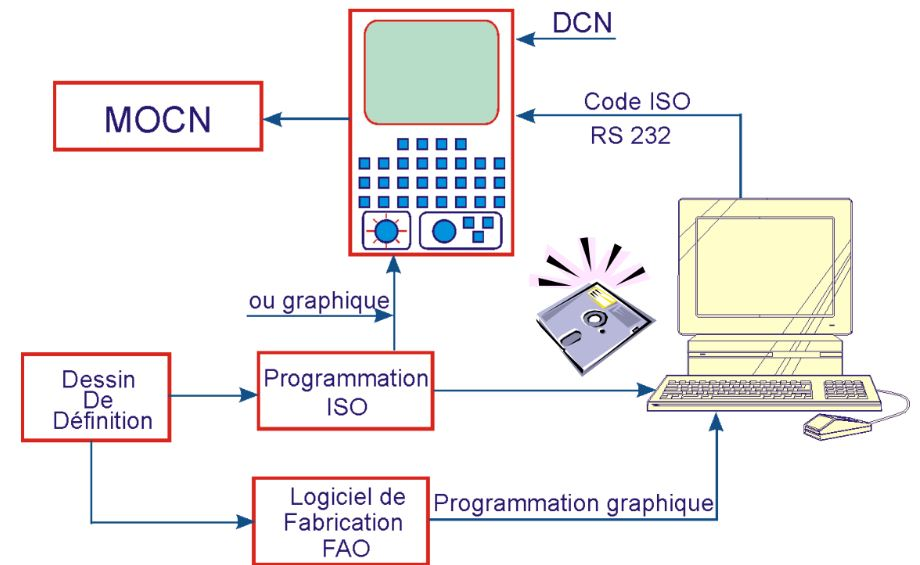
\includegraphics[width=0.7\textwidth]{Images/iso.JPG} % Include the figure image
	\caption{Chargement d'un programme dans une MOCN. Université des Sciences et de la Technologie d'Oran Mohamed-Boudiaf USTOMB}
	\label{iso3} % Unique label used for referencing the figure in-text
\end{figure}



Les machines ne sont pas comme nous, sans aucune perception de leur environnement elles sont dans le noir. Et nous leur demandons d'usiner avec une grande précision. Si on veut la longueur maximum d'une pièce de 20,001 mm mais que la pièce sortie mesure 20,002 : elle sera à jeter... Et on veut contrôler des vitesses très lentes ou très rapides (0,001 m/min à 130 m/min). \\



Alors dans tout ça, de quoi avons-nous besoin ? \\

\begin{theorem}
\begin{itemize}
    \item Un objet de départ dont on va enlever la matière : \textit{\textbf{Le brut de matière}} ;
    \item Des éléments pour enlever la matière : \textit{\textbf{Les outils}} ;
    \item De la force ! pour trancher, percer, tronçonner, fournie par : \textit{\textbf{Des moteurs}} ; 
    \item Oui mais si j'essaye de couper une feuille de papier avec des ciseaux, sans la tenir dans l'autre main c'est difficile, il faut donc que le \textit{Brut} soit solidement "attaché" : La \textit{\textbf{MIP}} et le \textit{\textbf{MAP}}\footnote{La MIP (MIse en Position) et le MAP (MAintient en Position) seront abordés plus tard dans l'année dans différents cours, mais surtout en industrialisation.}  ;
    \item  Pour faire la forme que l'on veut : \textit{\textbf{Une trajectoire}} ;
\end{itemize}
\end{theorem}

Dans la suite nous allons nous intéresser au dernier point. \textit{Repérer les éléments dans l'espace.} 

Pour usiner, nous avons besoin de plusieurs informations à chaque instant $t$, la position de l'outil qui usine, sa vitesse, son accélération, sa trajectoire. Ces informations doivent être calculées puis programmées dans la machine. Nous allons voir dans ce chapitre comment construire l'information : repérer les objets dans les MOCN.


\section{Outil mathématique pour futur.e.s ingénieur : Vous}

Un \textit{repère} sera présent pour \textbf{toutes} les études, analyses, interrogations que vous verrez. On ne peut pas faire sans. Sinon on ne serait pas capable de décrire ce que l'on voit sous forme mathématique et donc, impossible de programmer les machine. Un \textit{repère} est constitué de deux choses : Une $\mathcal{B}ase$ et une Origine. On l'écrit comme suit : $\mathcal{R}(0, \Vec{x}, \Vec{y}, \Vec{z})$.\\
On lit la phrase suivante : Voici $\mathcal{R}$, un repère constitué d'une origine $O$ et d'une $\mathcal{B}ase$ de vecteurs $\Vec{x}$, $\Vec{y}$, $\Vec{z}$. \\
La $\mathcal{B}ase$, c'est le tableau Excel infini, où sont présents tous les vecteur (en deux ou trois dimensions), mais ils ne peuvent pas être égaux. Par exemple, $\Vec{a}=\ \begin{Bmatrix} 1\\ 3 \end{Bmatrix} $ et $\Vec{b}=\ \begin{Bmatrix} 1\\ 3 \end{Bmatrix}$  ne peuvent pas être élus au rang de $\mathcal{B}ase$ car ils sont égaux. En revanche, dans la bibliothèque infinie il y a les vecteurs $\Vec{i}=\ \begin{Bmatrix} -1\\ 3 \\ 0 \end{Bmatrix} $ et $\Vec{j}=\ \begin{Bmatrix} -1\\ 0 \\ 3\end{Bmatrix}$ qui peuvent être choisi pour faire une base. \\



\begin{figure}[H] % Use [H] to suppress floating and place the figure/table exactly where it is specified in the text
	\centering % Horizontally center the figure on the page
	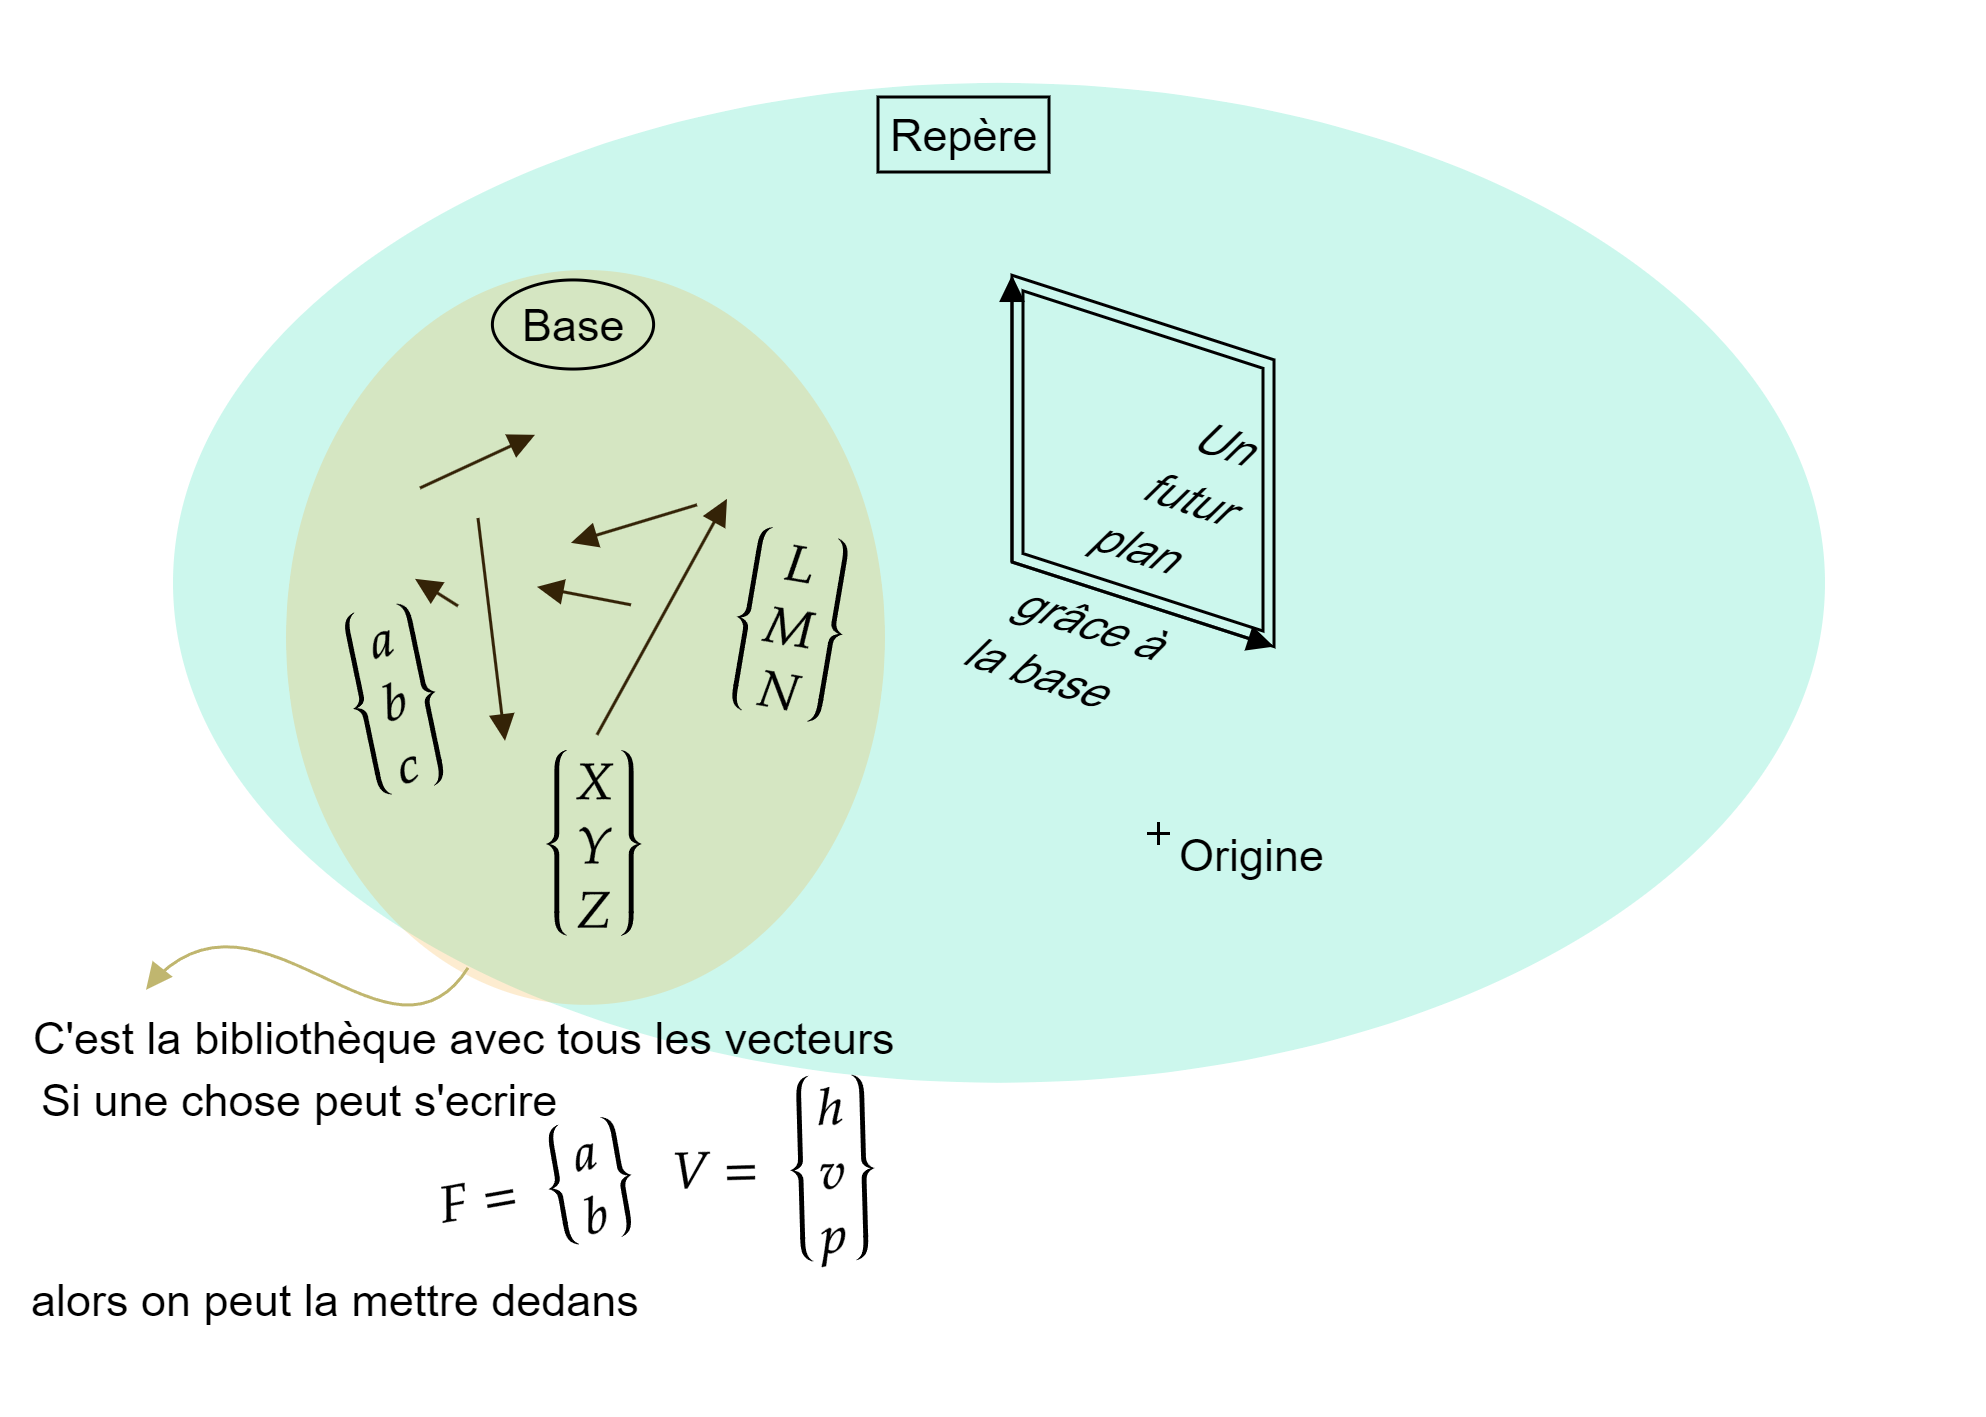
\includegraphics[width=1.1\textwidth]{Images/vect1.png} % Include the figure image
	\caption{Éléments pour construire un repère}
	\label{vect1} % Unique label used for referencing the figure in-text
\end{figure}


Un repère $\mathcal{R}$ est la donnée d’un point d'origine $\mathcal{O}$ et d’une base $\mathcal{B}$, permettant de repérer tous points de
l’espace par rapport à $\mathcal{O}$ (l'origine du repère). On décide que $\mathcal{O}$ est notre origine, on choisi deux vecteurs dans notre bibliothèque (sauf s'il sont égaux), on prend l'origine des deux vecteurs et on le colle sur notre point $\mathcal{O}$. Voilà, le repère est fait. \\

\begin{remark}
    En pratique, nous n'avons pas besoin de dire si un vecteur ou un repère est en 2 ou 3 dimensions. Un vecteur en 2 dimensions possède 2 données $\Vec{i}=\ \begin{Bmatrix} a\\ b \end{Bmatrix} $, il en possédera trois, pour la dimension trois : $\Vec{i}=\ \begin{Bmatrix} a\\ b \\ c \end{Bmatrix} $. De même, un repère en deux dimensions s'écriera $\mathcal{R}(0, \Vec{x}, \Vec{y})$, tandis-qu'un repère à trois dimensions s'écriera $\mathcal{R}(0, \Vec{x}, \Vec{y}, \Vec{z})$.    
\end{remark}

\begin{figure}[H] % Use [H] to suppress floating and place the figure/table exactly where it is specified in the text
	\centering % Horizontally center the figure on the page
	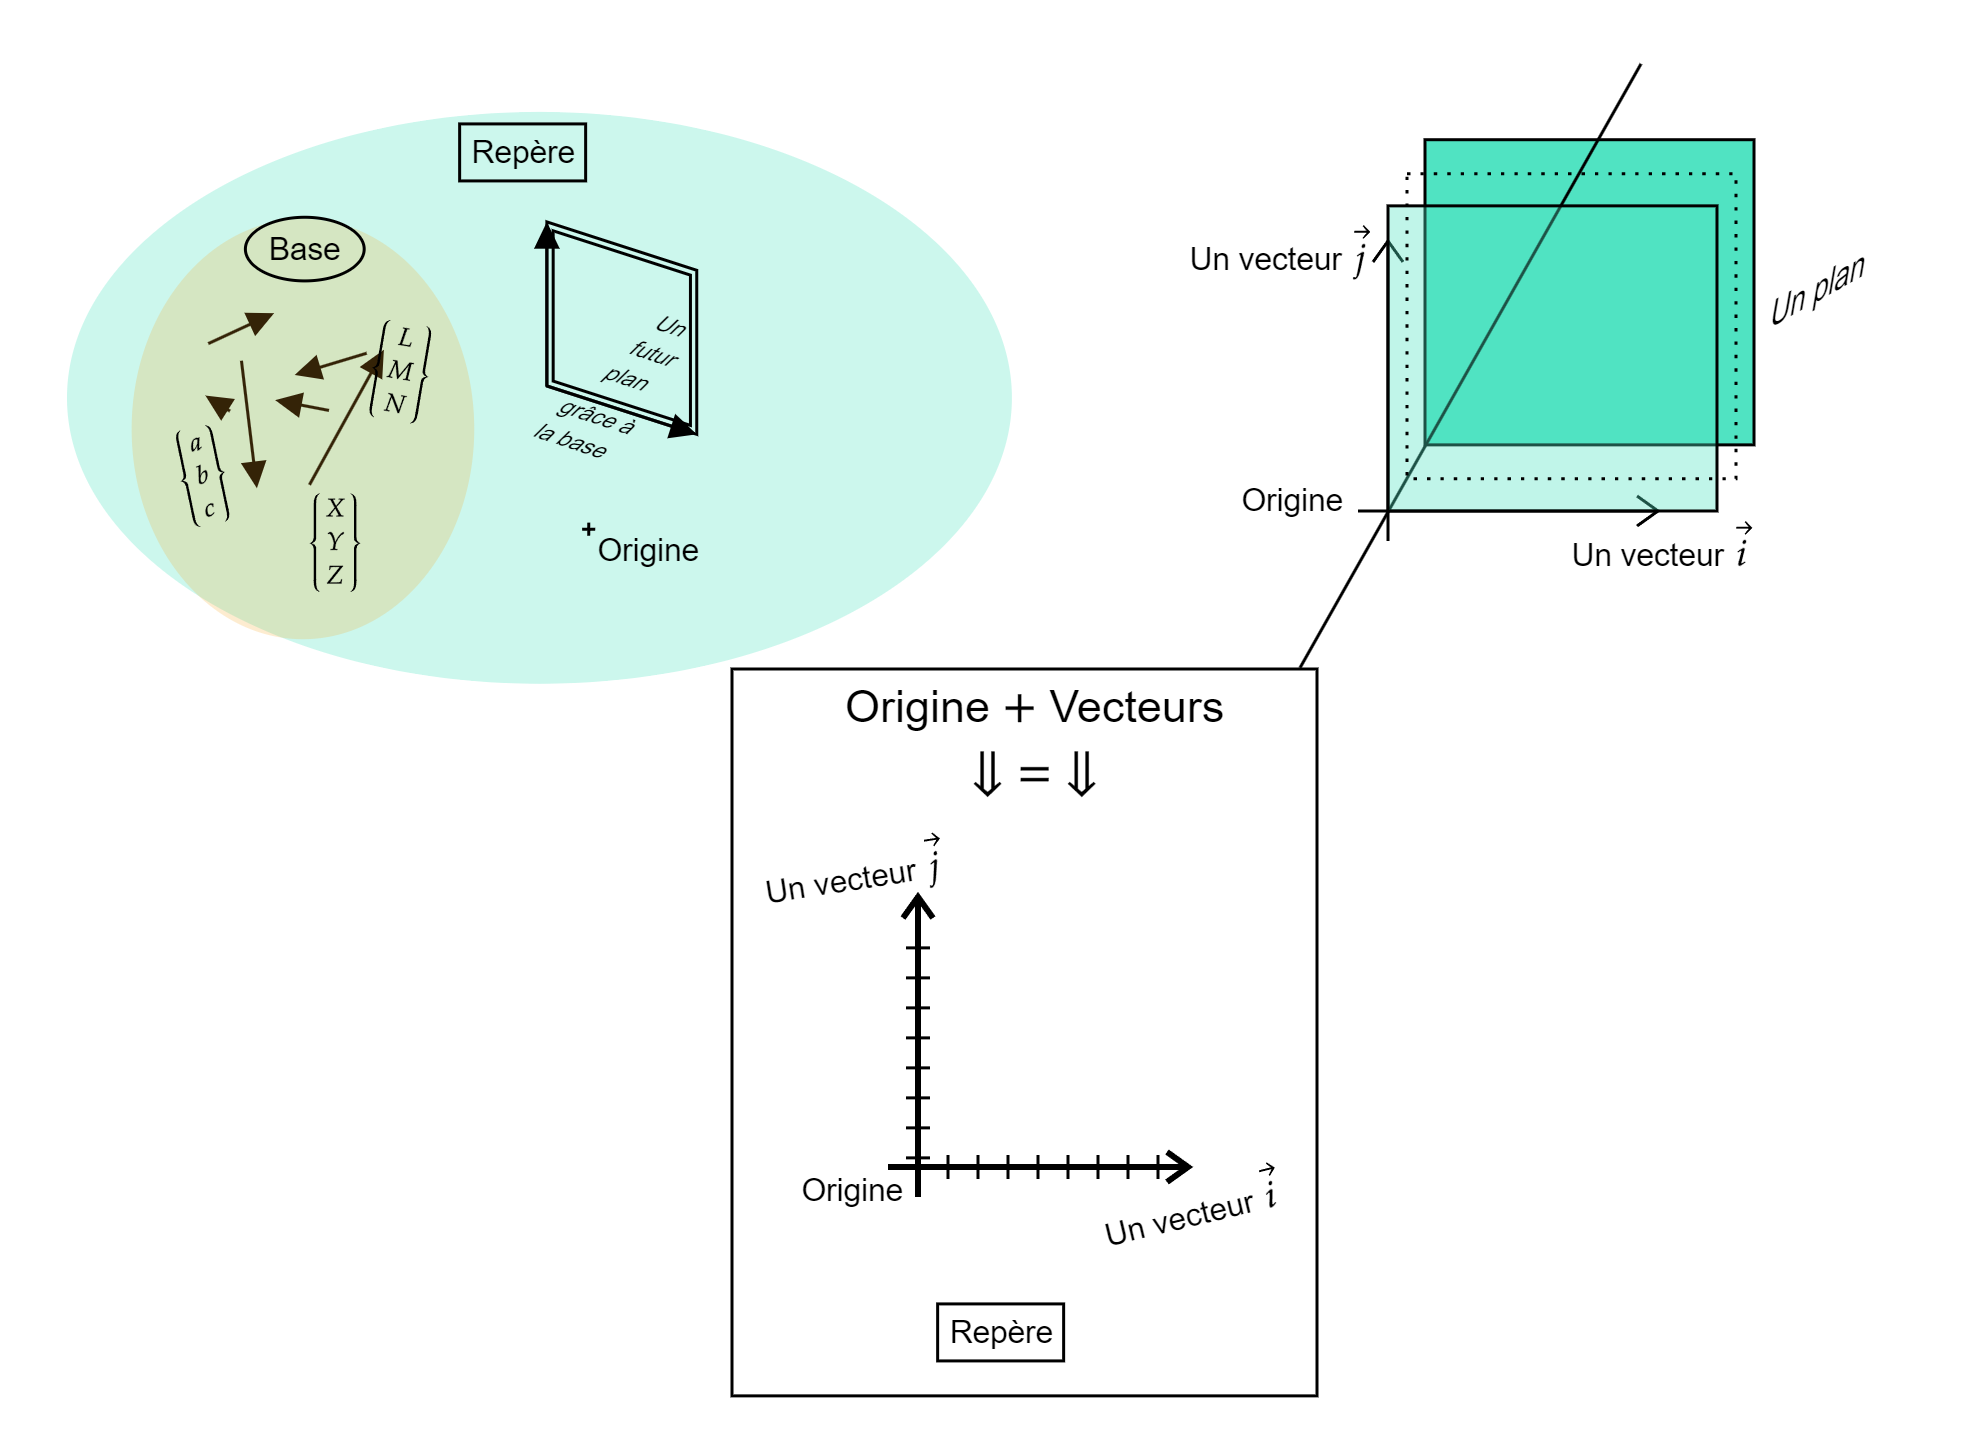
\includegraphics[width=1.1\textwidth]{Images/vect2.png} % Include the figure image
	\caption{Symbolisation d'un repère. Une fois une base (deux vecteurs) et une origine ($\mathcal{O}$) choisies, les deux vecteurs mis bout à bout forme un plan, et $\mathcal{O}$ nous sert à connaître n'importe quel point par rapport à lui.}
	\label{vect2} % Unique label used for referencing the figure in-text
\end{figure}

Maintenant que nous avons vu le cas général, nous allons voir les cas que vous croiserez en pratique. Que ce soit en théorie ou en pratique, en contrôle ou à l'examen, il y a quelque situation à connaître pour ne pas être surpris.e.

\section{Ortho-normé-direct}

Cette expression, vous la verrez beaucoup. Nous avons vu comment construire un repère, mais ceux qui seront utilisés pour les exercices ou en examens seront pour la plupart du temps construit pour être le plus simple possible. Nous allons détailler les repères principaux, qui sont orthogonaux, normés et directs.

\begin{figure}[H] % Use [H] to suppress floating and place the figure/table exactly where it is specified in the text
	\centering % Horizontally center the figure on the page
	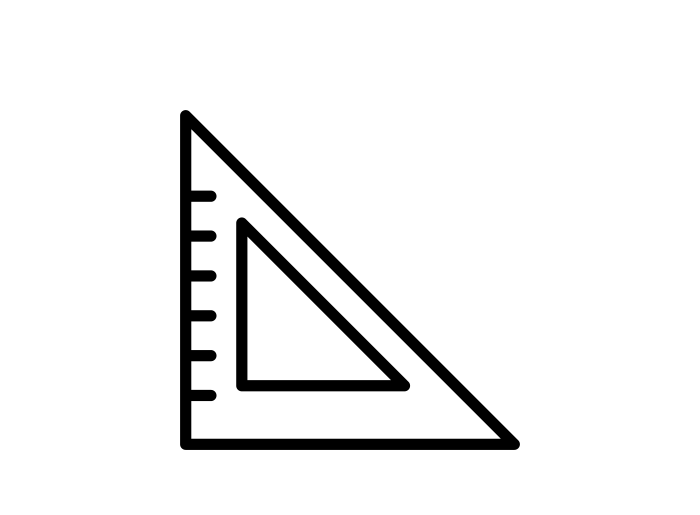
\includegraphics[width=0.25\textwidth]{Images/tri.png} % Include the figure image
    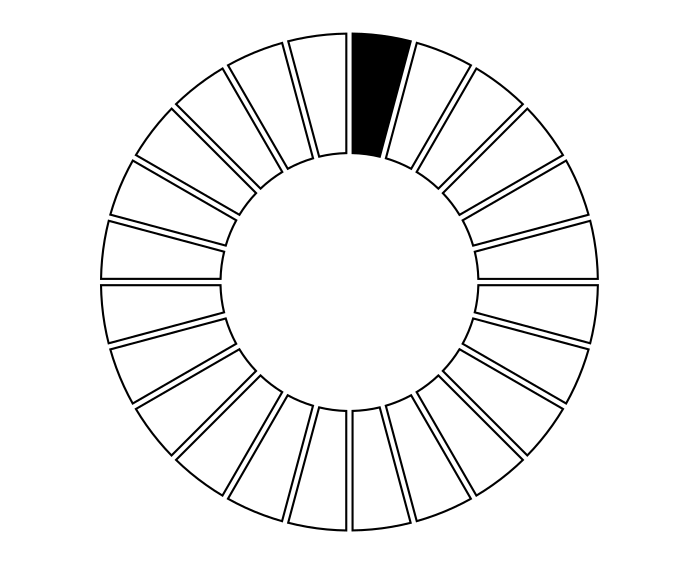
\includegraphics[width=0.2\textwidth]{Images/one.png} % Include the figure image
    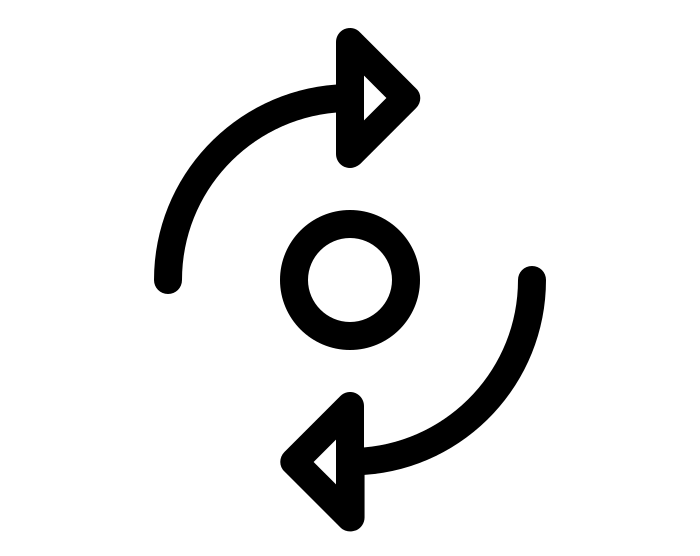
\includegraphics[width=0.2\textwidth]{Images/rot.png} % Include the figure image

\end{figure}




\subsection{Orthogonalité}
Les vecteurs que nous prenons dans notre bibliothèque (la $\mathcal{B}ase$) ne seront en général pas pris au hasard. On s'arrangera avoir deux vecteurs simplement perpendiculaires. 

\begin{figure}[H] % Use [H] to suppress floating and place the figure/table exactly where it is specified in the text
	\centering % Horizontally center the figure on the page
	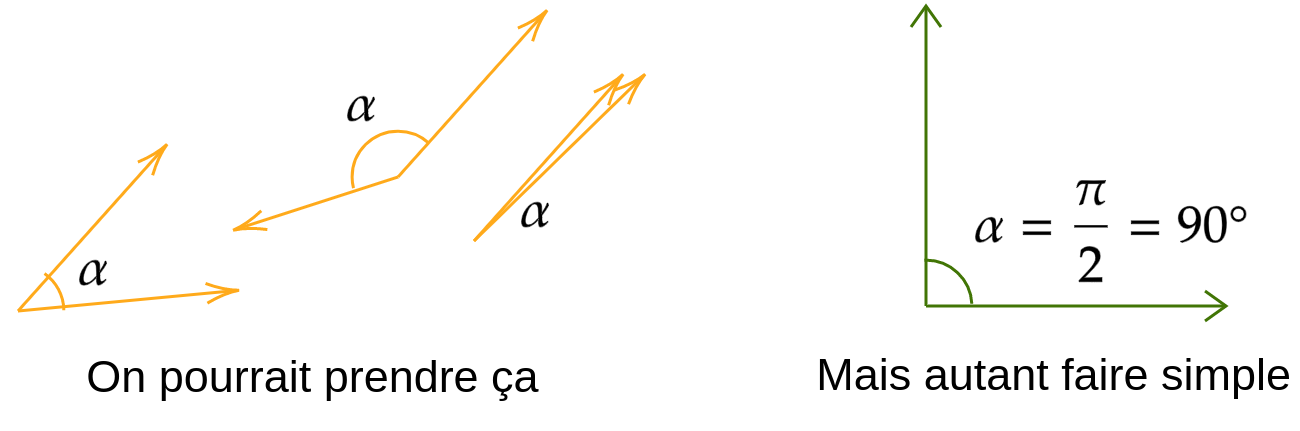
\includegraphics[width=0.8\textwidth]{Images/ortho1.png} % Include the figure image
	\label{ortho1} % Unique label used for referencing the figure in-text
\end{figure}

En sciences de l'ingénieur, on utilisera davantage certaines unités plutôt que d'autres. Notamment pour les rotations, les radians plutôt que les degrés. Une rotation d'un demi tour ($180^{\circ}$) sera égal à $\pi$ ce qui simplifiera grandement les calculs.







\subsection{Normé}

Une autre simplification est la normalisation des vecteurs utilisés pour construire une base. 
\begin{figure}[H] % Use [H] to suppress floating and place the figure/table exactly where it is specified in the text
	\centering % Horizontally center the figure on the page
	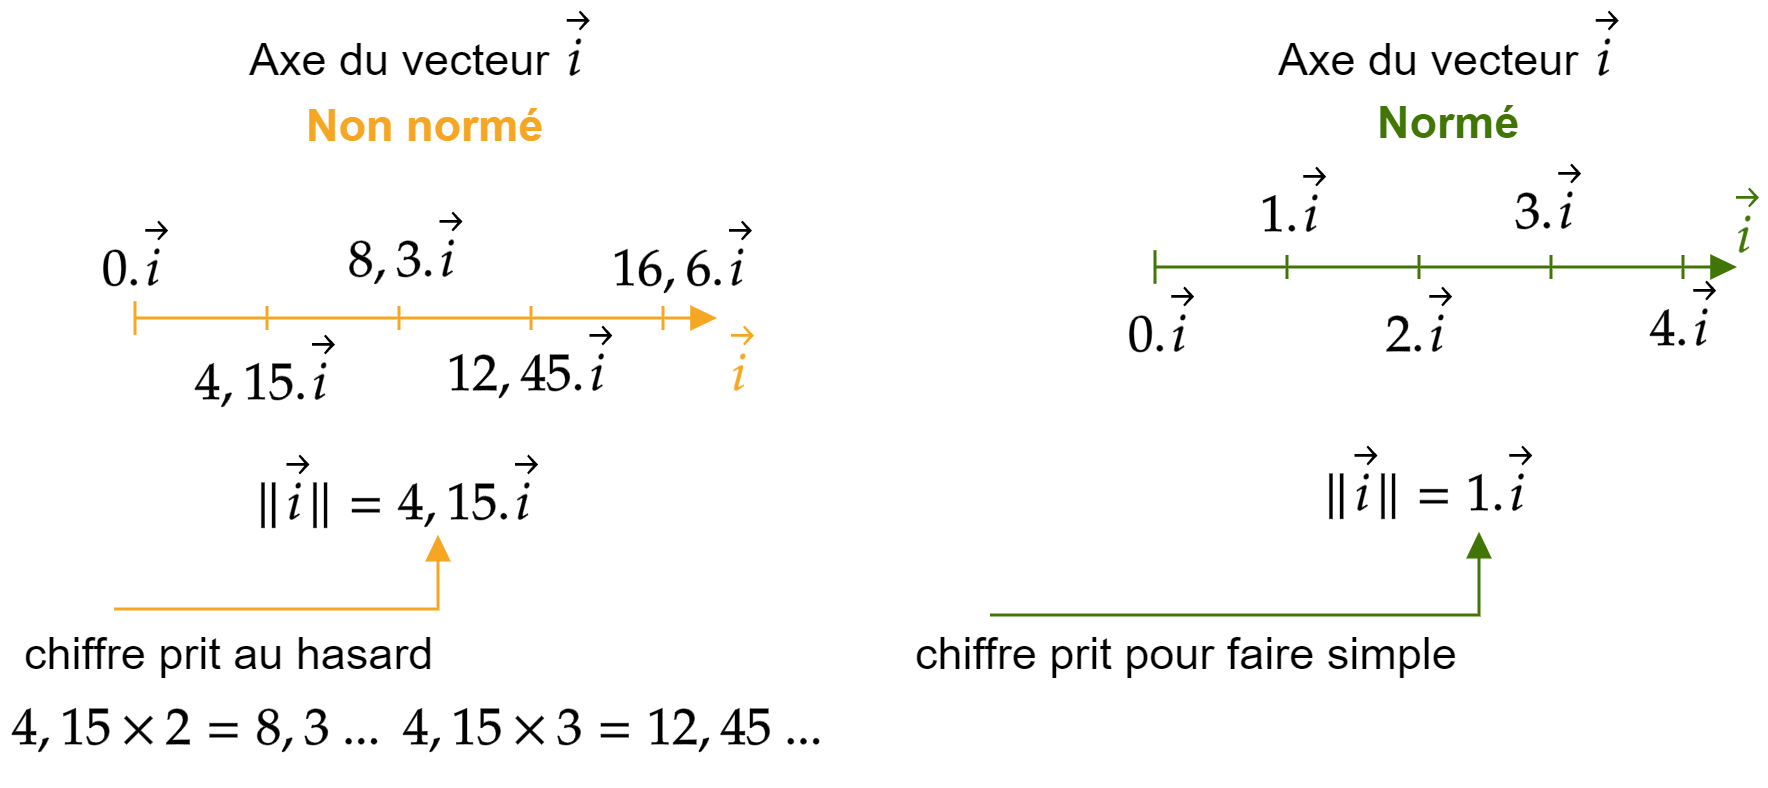
\includegraphics[width=1\textwidth]{Images/norme2.png} % Include the figure image
	\caption{Construction d'une base avec des vecteurs à norme unitaire.}
	\label{norme2} % Unique label used for referencing the figure in-text
\end{figure}

La distance entre chaque trait d'un repère dit normé est de \textit{une} unité. L'aspect plus scientifique des \textit{vecteurs unitaires} sera détaillé dans le chapitre [\ref{Vecteurs}] dédié.

\begin{definition}\index{Vecteur unitaire}
Un vecteur qui possède une norme de une unité est appelé \textbf{vecteur unitaire}. En mathématique, la norme de quelque chose s'écrit $ \Vert quelque chose \Vert $ On écrira donc : $ \Vert \Vec{u} \Vert = 1\ $
\end{definition}




\subsection{Direct}

En choisissant un repère dit \textit{direct}, on choisira une fois pour toute, le sens \textbf{positif} de rotation entre les axes. En grande majorité, on prendra le sens \textbf{anti-horaire}, donc \textbf{trigonométrique}. Cela simplifiera les calculs, notamment pour toutes les formules de trigonométrie. De plus, il est important d'avoir un outil commun, par exemple pour décrire la rotation d'une vis dans son logement les calculs négatifs ou positifs peuvent décrire un vissage ou dévissage et une erreur de compréhension doit être évitée.

\begin{figure}[H] % Use [H] to suppress floating and place the figure/table exactly where it is specified in the text
	\centering % Horizontally center the figure on the page
	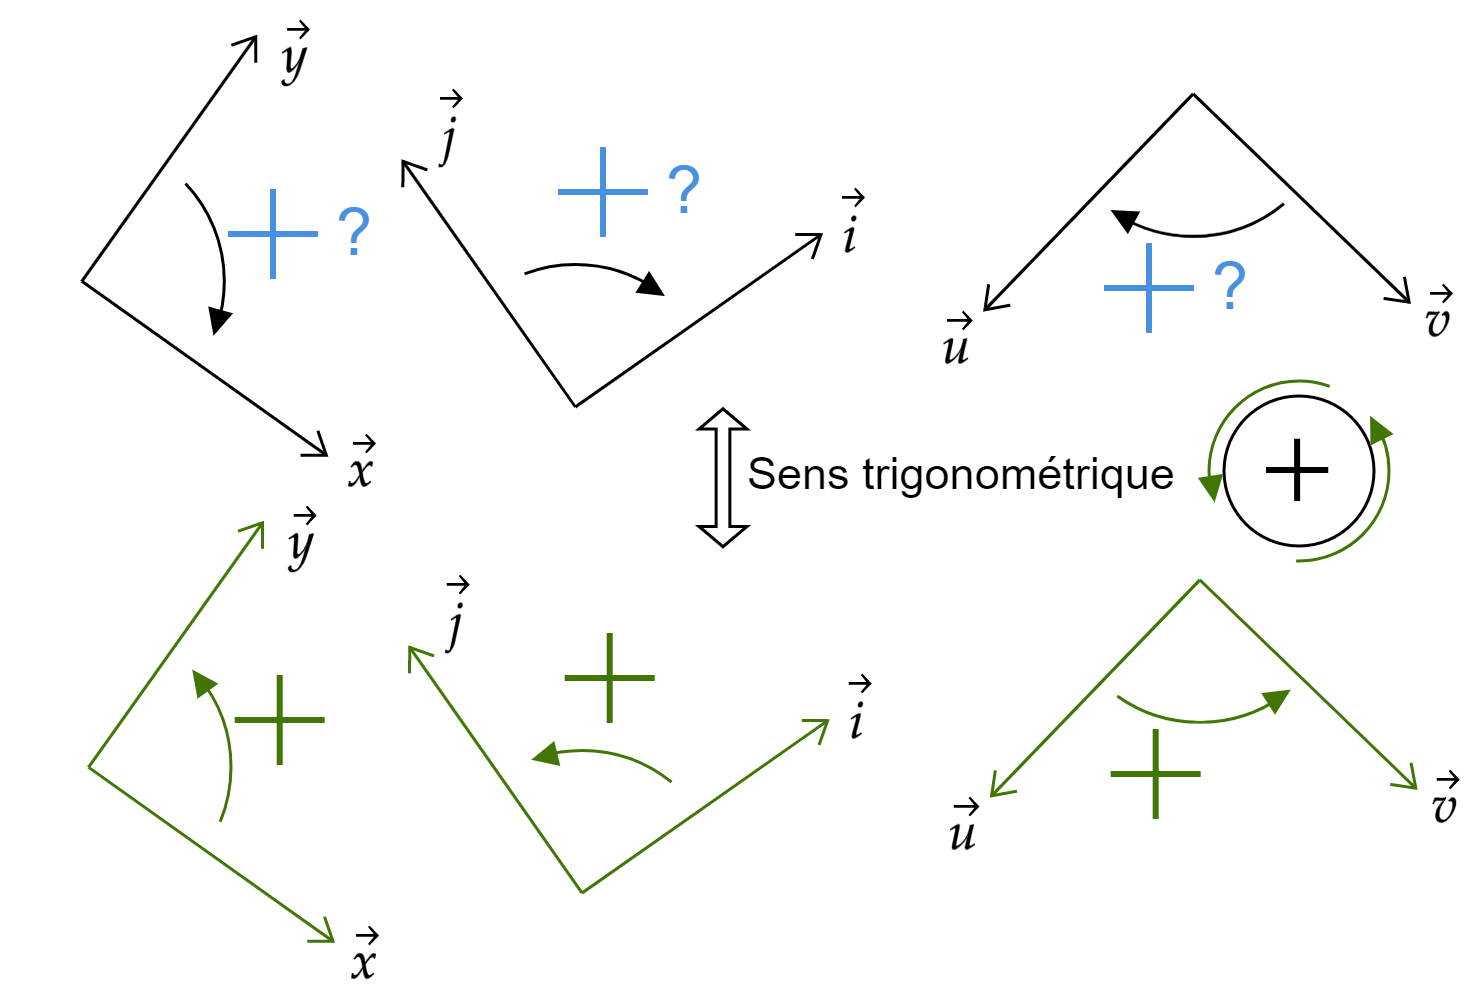
\includegraphics[width=0.8\textwidth]{Images/direct1.png} % Include the figure image
	\caption{Construction d'une base suivant le sens trigonométrique.}
	\label{direct1} % Unique label used for referencing the figure in-text
\end{figure}



\begin{theorem}
Au final, on aura donc un repère qui en général, se composera de deux vecteurs non égaux et unitaires, qui seront mis bout à bout et perpendiculaires. L'endroit de leur rencontre sera le point d'origine du repère. Et le sens sera positif quand on suivra le sens trigonométrique.
\end{theorem}

\begin{figure}[H] % Use [H] to suppress floating and place the figure/table exactly where it is specified in the text
	\centering % Horizontally center the figure on the page
	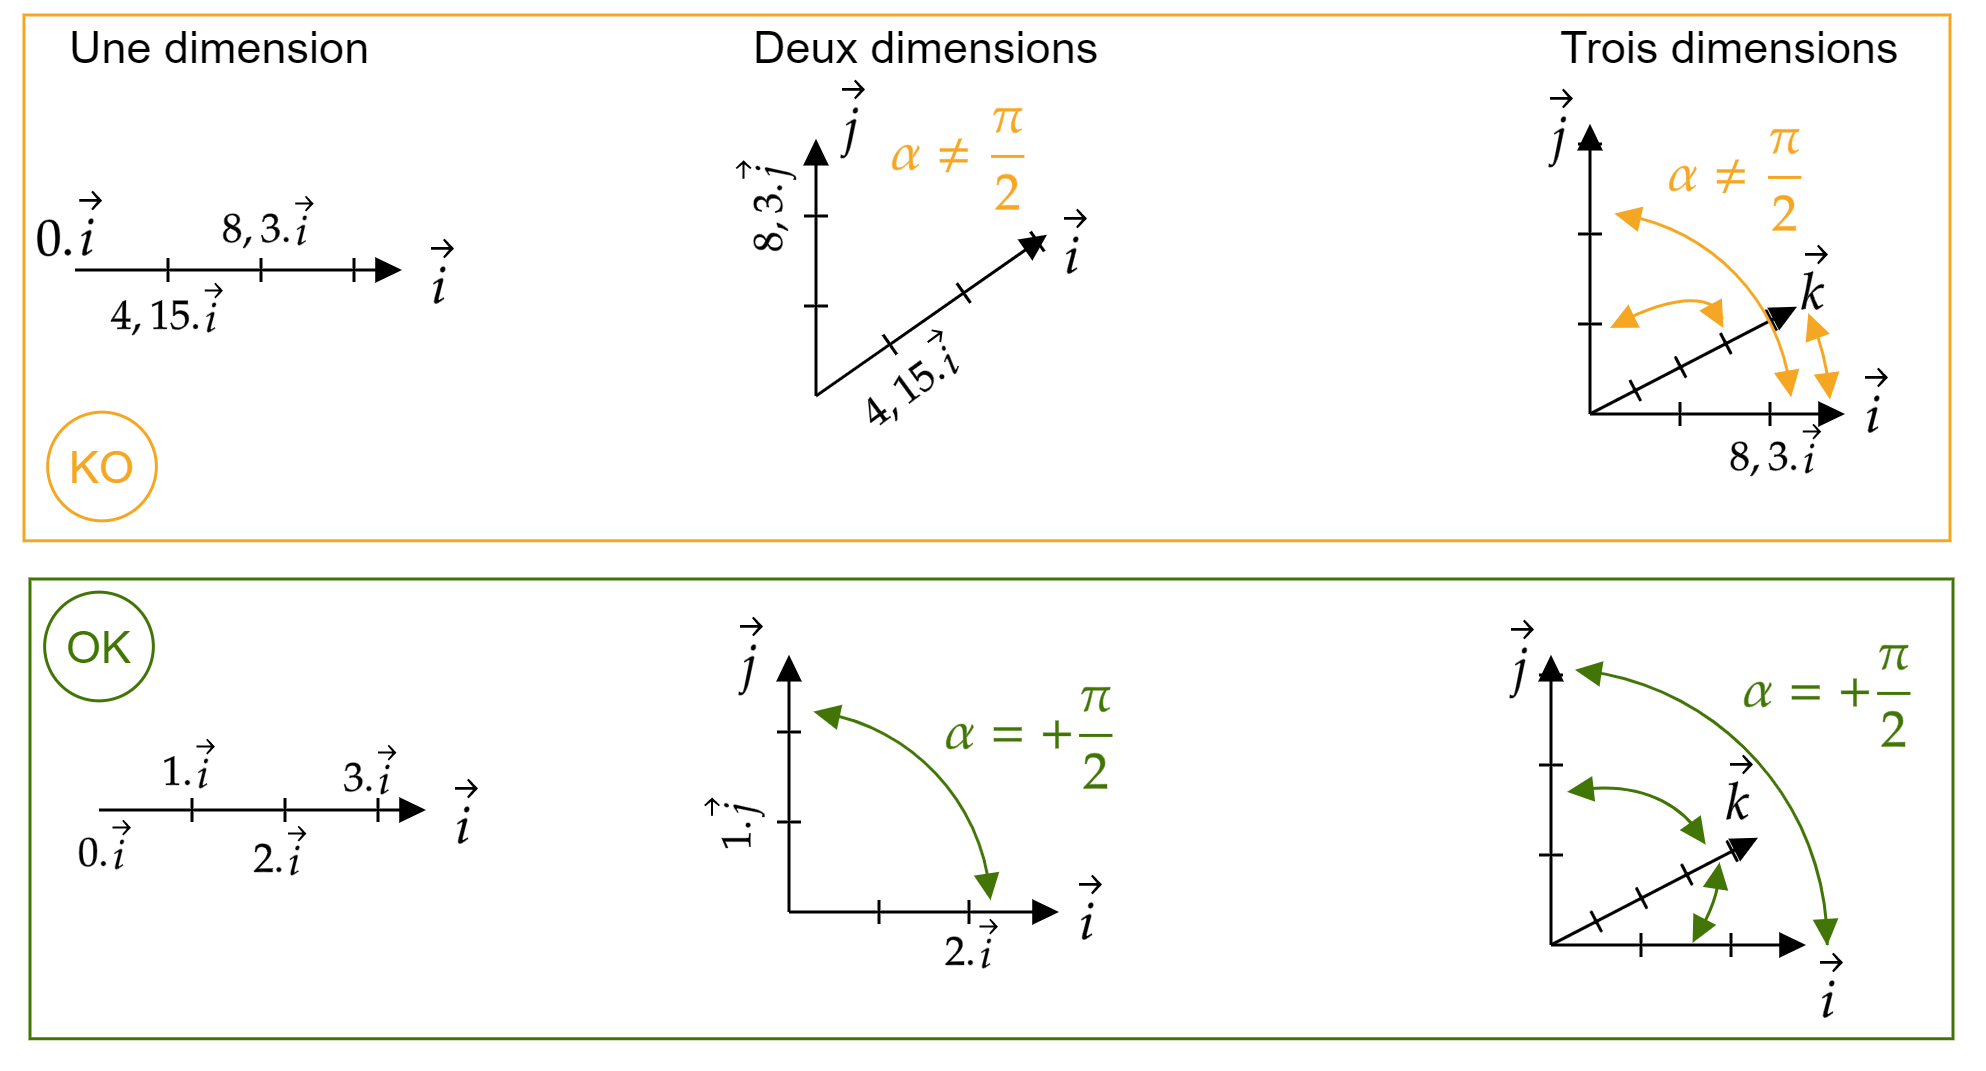
\includegraphics[width=1\textwidth]{Images/repere2.png} % Include the figure image
	\caption{Construction d'un repère pour dimension 1, 2 et 3.}
	\label{repere2} % Unique label used for referencing the figure in-text
\end{figure}

Pour la commodité des exercices, vous pourrez croiser plusieurs type de schéma de repère. Retenez les avec attention pour prendre l'habitude de leurs différences. 


\begin{figure}[H] % Use [H] to suppress floating and place the figure/table exactly where it is specified in the text
	\centering % Horizontally center the figure on the page
	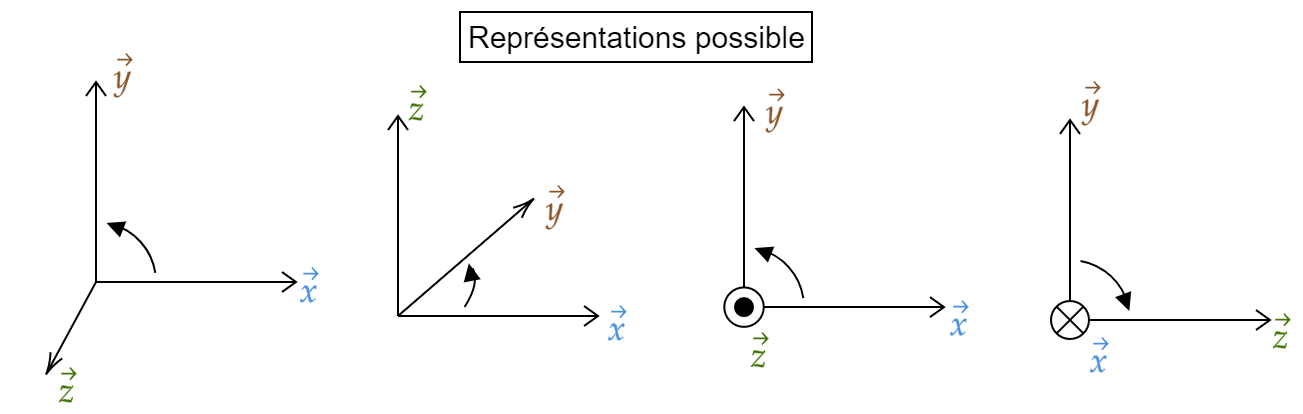
\includegraphics[width=1\textwidth]{Images/repere3.png} % Include the figure image
	\caption{Schémas type de repères en fonction du sens direct.}
	\label{repere3} % Unique label used for referencing the figure in-text
\end{figure}

Pour respecter le sens direct des repères, on nom des axes doit être adapté, comme sur le dernier schéma de la figure [\ref{repere3}]. Il faudra toujours garder la suite $\Vec{x}, \Vec{y}, \Vec{z}$ ou $\Vec{u}, \Vec{v}, \Vec{w}$ etc.


Dans les conditions d'un repère otho-normé-direct, on pourra utiliser les relations trigonométriques suivantes :

$\displaystyle \cos( \theta -\pi ) =\ -\cos( \theta )$ et $\displaystyle \sin( \theta +\pi ) =-\sin( \theta )$ \\

$\displaystyle \cos( \pi -\theta ) =-\cos( \theta )$ et $\displaystyle \sin( \pi -\theta ) =\sin( \theta )$ \\

$\displaystyle \cos( -\theta ) =\cos( \theta )$ et $\displaystyle \sin( -\theta ) =-\sin( \theta )$ \\

$\displaystyle \cos\left(\frac{\pi }{2} -\theta \right) =\sin( \theta )$ et $\displaystyle \sin\left(\frac{\pi }{2} -\theta \right) =\cos( \theta )$ \\

$\displaystyle \cos\left( \theta +\frac{\pi }{2}\right) =-\sin( \theta )$ et $\displaystyle \sin\left( \theta +\frac{\pi }{2}\right) =\cos( \theta )$ 

\section{Référentiel}

\begin{definition}\index{Référentiel}
Un Référentiel est l'association d'un repère auquel on ajoute on ajoute le temps $t$ (avec la seconde comme unité par exemple).
\end{definition}

\begin{figure}[H] % Use [H] to suppress floating and place the figure/table exactly where it is specified in the text
	\centering % Horizontally center the figure on the page
	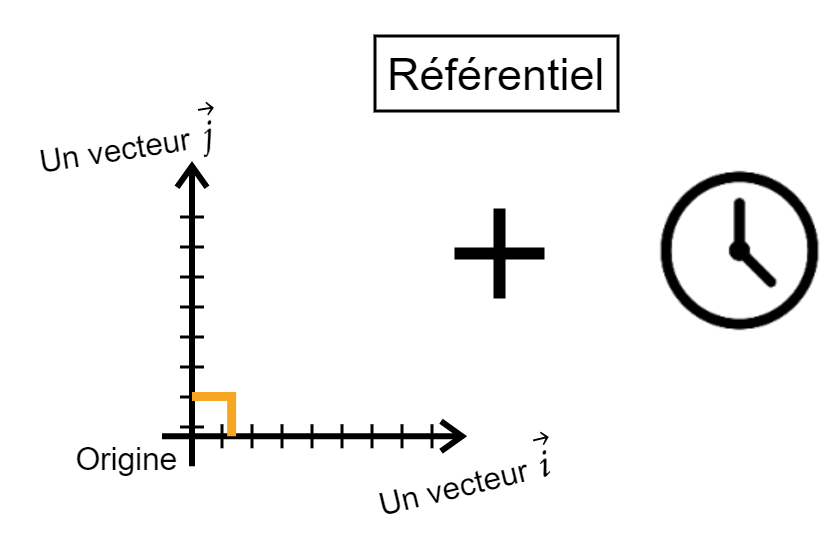
\includegraphics[width=0.5\textwidth]{Images/ref1.png} % Include the figure image
	\caption{Définition d'un référentiel}
	\label{ref1} % Unique label used for referencing the figure in-text
\end{figure}

Pour nous permettre d'étudier les phénomènes physiques, on prendra l'habitude de s'imaginer dans un référentiel. On peut ressentir l'effet des référentiels différents dans le métro ou le RER. Il arrive de ne pas savoir si c'est notre wagon qui est entrain de partir, ou si c'est celui d'en face. Parce qu'on ne nous dit pas ce qui est fixe par rapport à nous, et ce qui est mobile. En effet, tout ce que nous connaissons est en perpétuel mouvement et peut influencer toutes les observations. Notre planète tourne sur elle-même et se déplace autour du Soleil, qui est lui-même en mouvement à 850 000 $km/h$ dans une galaxie qui se déplace à plus de $631\pm 20 km/s$ attirée par la lointaine concentration de masse Shapley\footnote{Article scientifique : The dipole repeller, Yehuda Hoffman, Daniel Pomarède, R. Brent Tully \& Hélène M. Courtois. https://www.nature.com/}.

Pour pouvoir représenter et étudier un mouvement il faut admettre que son cadre d'observation est fixe pour ne pas qu'il influe sur le phénomène à étudier. C'est pour cela que l'on utilise un référentiel. Il existe plein de référentiel, mais nos études se limiterons en général à des objets très petits ou des vitesses négligeables par rapport à celle de la lumière. Ce qu'il faut retenir c'est surtout le fait qu'un référentiel c'est l'ajout supplémentaire d'une coordonnées de temps. On a donc au final 2 ou 3 coordonnées de position et une coordonnées de temps. Attention, la coordonnées de temps fait souvent partie des coordonnées utilisées sur le repère. Par exemple, si on regarde la hauteur et la distance d'une pomme qui est entrain de tomber, on aura deux coordonnées de position (qui elles même dépendent du temps) et une coordonnées de temps. On a seulement deux coordonnées pour l'analyse voulue mais le temps est toujours là.



\begin{figure}[H] % Use [H] to suppress floating and place the figure/table exactly where it is specified in the text
	\centering % Horizontally center the figure on the page
	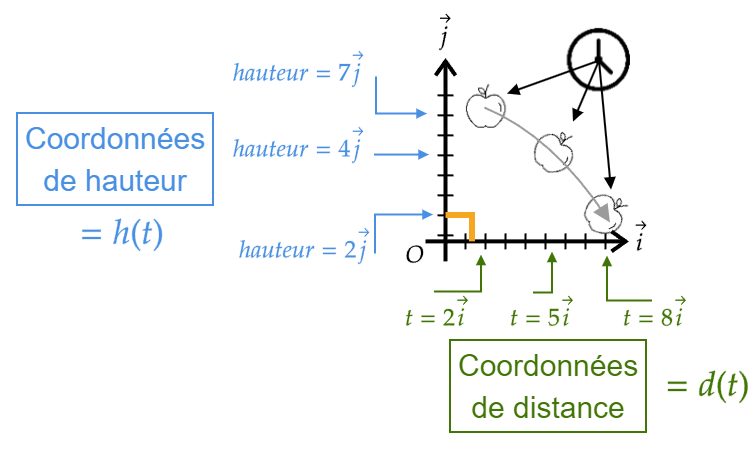
\includegraphics[width=1\textwidth]{Images/ref2.png} % Include the figure image
	\caption{Référentiel disposant de deux coordonnées, la hauteur $h(t)$ suivant $\Vec{j}$ et la distance $d(t)$ suivant $\Vec{i}$.}
	\label{ref2} % Unique label used for referencing the figure in-text
\end{figure}

Sur la figure [\ref{ref2}] on peut par exemple dire que la hauteur doit être en mètre et le temps en seconde. 

\section{Coordonnées}
A ce stade, nous avons un espace qui n'attend plus d'avoir des éléments à l'intérieur. Avec le repère orthonormé direct qu'on utilise, nous pouvons maintenant repérer des points, décrire le mouvement des vents, voir la force engendrée par un barrage ou la trajectoire d'un outil dans une MOCN. Mais encore une fois, on ne peut pas démarrer directement, il y a en effet différents \textit{systèmes} de coordonnées. Comme on choisi son mode de transport en fonction de notre destination, le système de coordonnée sera choisi en fonction de ce qu'il faudra traiter.

\subsection{Coordonnées cartésiennes}
Ce système de coordonnées est le plus rependus, il est facile à visualiser et vous l'utilisez énormément. Le repère que l'on prend nous donne un espace où des points pourront être posé et repéré par rapport à l'origine et aux axes.

Nous partons d'un repère $\mathcal{R}$ muni d'une $\mathcal{B}ase(\Vec{x}, \Vec{y}, \Vec{z})$ : $\mathcal{R}(O, \Vec{x}, \Vec{y}, \Vec{z}$).

On repère simplement les points du système de coordonnées cartésien par leur coordonnées selon chaque axes. Si on se place en 3 dimensions, un point aura donc trois données.

\begin{figure}[H] % Use [H] to suppress floating and place the figure/table exactly where it is specified in the text
	\centering % Horizontally center the figure on the page
	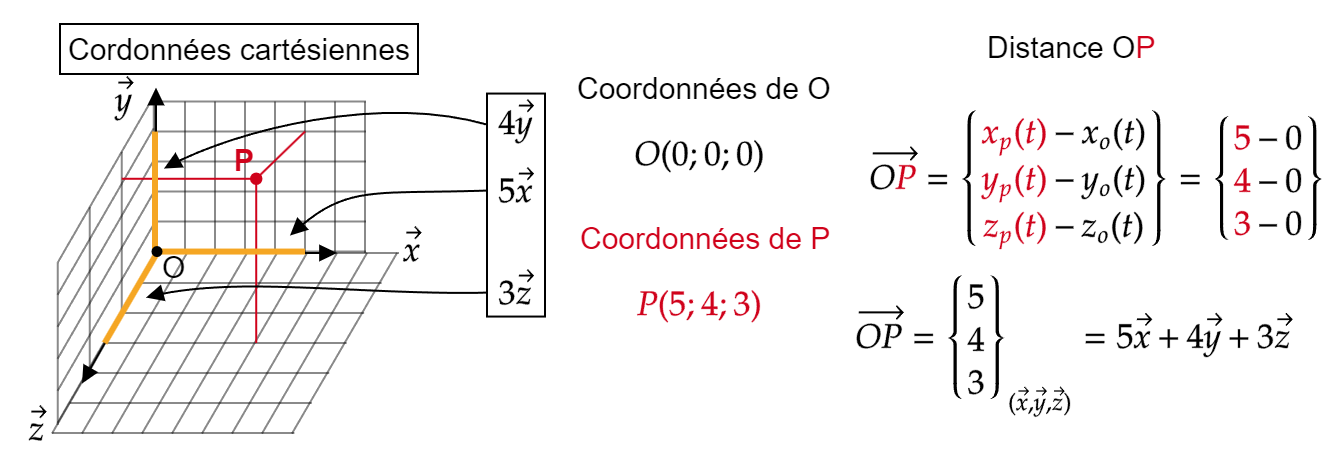
\includegraphics[width=1\textwidth]{Images/cart0.png} % Include the figure image
	\caption{Coordonnées cartésiennes : Repérage d'un point P.}
	\label{cart0} % Unique label used for referencing the figure in-text
\end{figure}

La figure [\ref{cart0}] prendre l'exemple d'un point P avec des valeurs algébriques, dans le cas général on peut noter la distance $\Vec{OP}$ comme suit : $\Vec{OP}=x\Vec{x}+y\Vec{y}+z\Vec{z}$ avec x, y et z n'importe quelle valeur.

\begin{figure}[H] % Use [H] to suppress floating and place the figure/table exactly where it is specified in the text
	\centering % Horizontally center the figure on the page
	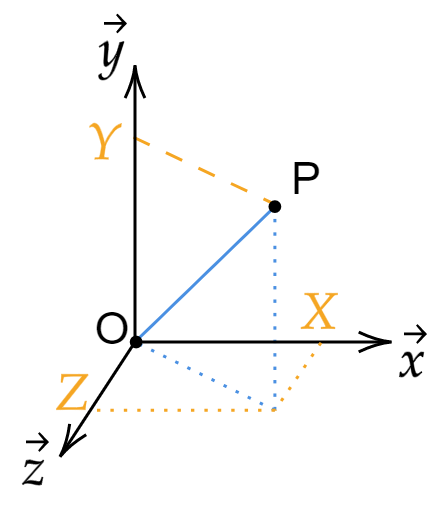
\includegraphics[width=0.3\textwidth]{Images/cart1.png} % Include the figure image
	\caption{Coordonnées cartésiennes : cas général.}
	\label{cart1} % Unique label used for referencing the figure in-text
\end{figure}

Concrètement, c'est un système de coordonnées que vous manipulerez pour des études sur fraiseuses ou centres d'usinage car il s'y prête très bien.

\begin{remark}
    Attention, il est facile d'être pertubé.e sur certaines notations. Quand on écrit $\Vec{OP}=x\Vec{x}+y\Vec{y}+z\Vec{z}$ il faut bien faire la différence entre les vecteurs unitaires ($\Vec{x}, \Vec{y}, \Vec{z}$)et les valeurs ($x, y, z$) qui peuvent avoir le même nom dans certain exercice.
\end{remark}

\begin{figure}[H] % Use [H] to suppress floating and place the figure/table exactly where it is specified in the text
	\centering % Horizontally center the figure on the page
	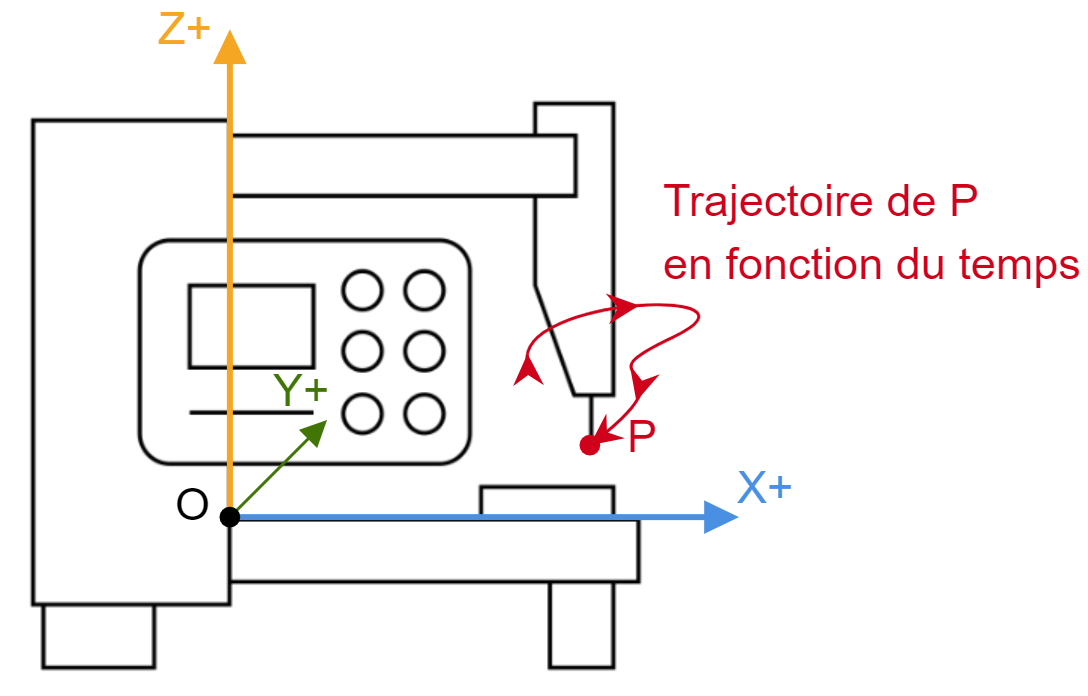
\includegraphics[width=0.8\textwidth]{Images/cart2.png} % Include the figure image
	\caption{Utilisation des coordonnées cartésiennes pour une fraiseuse.}
	\label{cart2} % Unique label used for referencing the figure in-text
\end{figure}

\subsection*{Programmation d'une trajectoire sur fraiseuse en coordonnées cartésiennes}



\begin{figure}[H] % Use [H] to suppress floating and place the figure/table exactly where it is specified in the text
	\centering % Horizontally center the figure on the page
	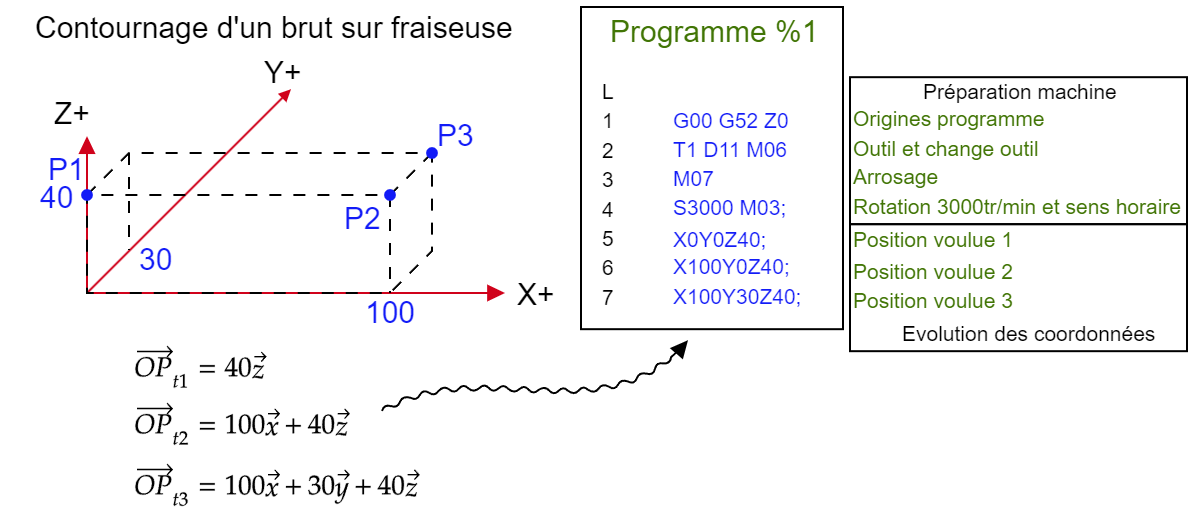
\includegraphics[width=1\textwidth]{Images/cart3.png} % Include the figure image
	\caption{Calcul des coordonnées cartésiennes à programmer pour une fraiseuse.}
	\label{cart3} % Unique label used for referencing the figure in-text
\end{figure}

En apprenant le vocabulaire de la programmation ISO, vous serez facilement programmer n'importe quelle trajectoire. Bien sur il faudra ajouter des notions programme que nous n'avons pas encore vue tels que les accélérations/ralentissement, correction de rayon etc.


\subsection*{Programmation d'une trajectoire sur tour en coordonnées cartésiennes}


\begin{figure}[H] % Use [H] to suppress floating and place the figure/table exactly where it is specified in the text
	\centering % Horizontally center the figure on the page
	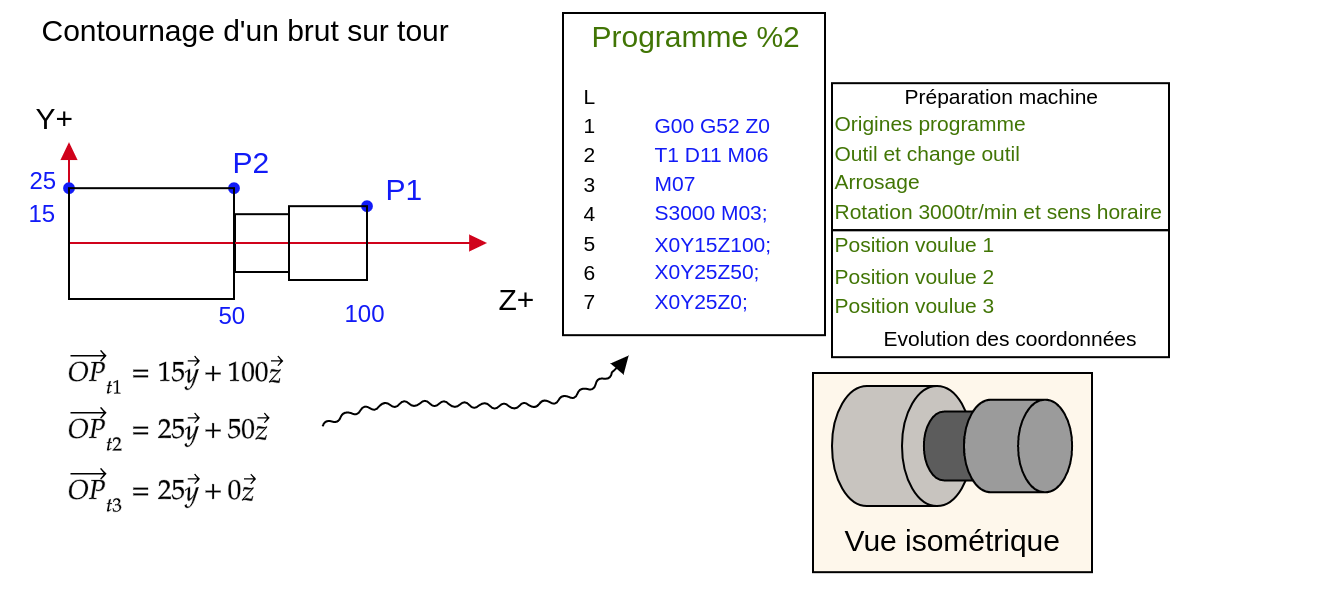
\includegraphics[width=1\textwidth]{Images/cart4.png} % Include the figure image
	\caption{Calcul des coordonnées cartésiennes à programmer pour un chariotage/dressage sur un tour.}
	\label{cart4} % Unique label used for referencing the figure in-text
\end{figure}

\begin{remark}
    Sur un tour, on pourrait s'attendre à choisir des coordonnées polaires ou cylindriques cependant, l'outil qui vient enlever la matière pour une pièce de révolution est toujours sur le même plan.

    \begin{figure}[H] % Use [H] to suppress floating and place the figure/table exactly where it is specified in the text
	\centering % Horizontally center the figure on the page
	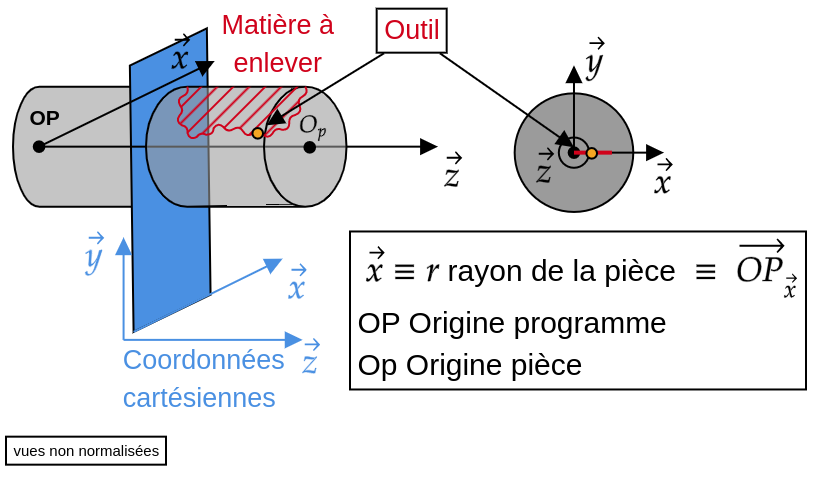
\includegraphics[width=1\textwidth]{Images/coord1.png} % Include the figure image
\end{figure}

Pour usiner une pièce de révolution sur un tour 2 axes, l'outil ne peut bouger que sur l'axe $\Vec{z}$ et s'approcher ou s'éloigner de celui-ci sur l'axe $\Vec{x}$\footnote{Il translate grâce à une liaison roue-vis sans fin, d'un moteur, et d'un codeur absolu pour repérer la position et la vitesse de translation.} L'axe $\Vec{z}$ est lié à la longueur de la pièce, on y contrôle la vitesse d'avance ($V_f$\footnote{f pour forward ?}) et la longueur qu'on veut enlever au brut. L'axe $\Vec{x}$ est lié au diamètre de la pièce, on y contrôle plusieurs éléments important comme la profondeur de passe ($A_p$), la vitesse de coupe ($V_c$) ou plus généralement la forme de la pièce.


\end{remark}


\begin{Exercice}


\tikzset{every picture/.style={line width=0.75pt}} %set default line width to 0.75pt        

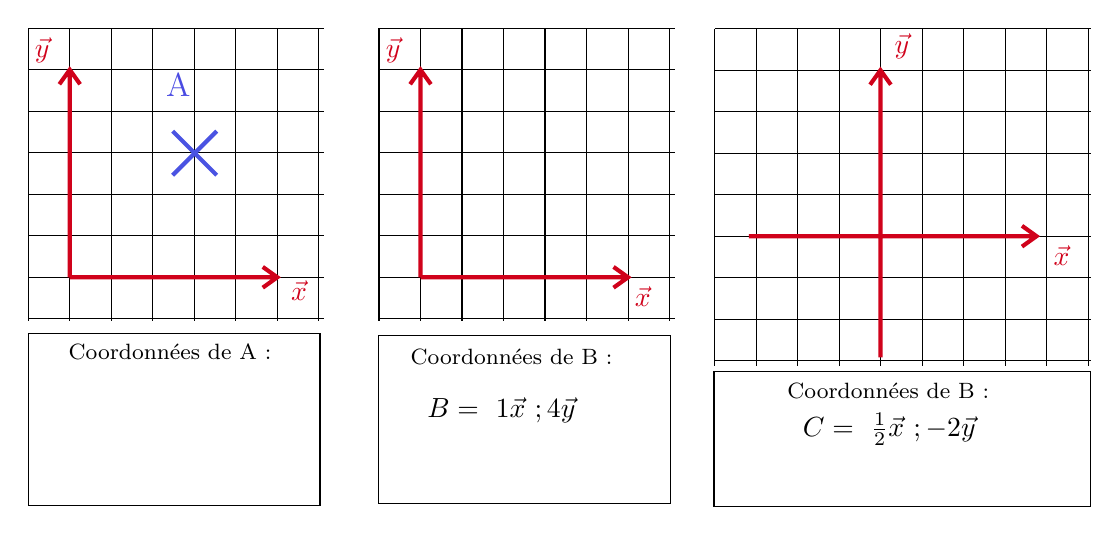
\begin{tikzpicture}[x=0.75pt,y=0.75pt,yscale=-1,xscale=1]
%uncomment if require: \path (0,240); %set diagram left start at 0, and has height of 240

%Shape: Grid [id:dp3932706137193831] 
\draw  [draw opacity=0] (1.2,4.2) -- (143.6,4.2) -- (143.6,145.2) -- (1.2,145.2) -- cycle ; \draw   (1.2,4.2) -- (1.2,145.2)(21.2,4.2) -- (21.2,145.2)(41.2,4.2) -- (41.2,145.2)(61.2,4.2) -- (61.2,145.2)(81.2,4.2) -- (81.2,145.2)(101.2,4.2) -- (101.2,145.2)(121.2,4.2) -- (121.2,145.2)(141.2,4.2) -- (141.2,145.2) ; \draw   (1.2,4.2) -- (143.6,4.2)(1.2,24.2) -- (143.6,24.2)(1.2,44.2) -- (143.6,44.2)(1.2,64.2) -- (143.6,64.2)(1.2,84.2) -- (143.6,84.2)(1.2,104.2) -- (143.6,104.2)(1.2,124.2) -- (143.6,124.2)(1.2,144.2) -- (143.6,144.2) ; \draw    ;
%Shape: Axis 2D [id:dp39250656962639074] 
\draw [color={rgb, 255:red, 208; green, 2; blue, 27 }  ,draw opacity=1 ][line width=1.5]  (21.2,124.2) -- (121.2,124.2)(21.2,24.2) -- (21.2,124.2) -- cycle (114.2,119.2) -- (121.2,124.2) -- (114.2,129.2) (16.2,31.2) -- (21.2,24.2) -- (26.2,31.2)  ;
\draw  [color={rgb, 255:red, 74; green, 83; blue, 226 }  ,draw opacity=1 ][line width=1.5]  (70.79,53.79) -- (92.01,75.01)(92.01,53.79) -- (70.79,75.01) ;
%Shape: Grid [id:dp9415796246319506] 
\draw  [draw opacity=0] (170.2,4.2) -- (312.6,4.2) -- (312.6,145.2) -- (170.2,145.2) -- cycle ; \draw   (170.2,4.2) -- (170.2,145.2)(190.2,4.2) -- (190.2,145.2)(210.2,4.2) -- (210.2,145.2)(230.2,4.2) -- (230.2,145.2)(250.2,4.2) -- (250.2,145.2)(270.2,4.2) -- (270.2,145.2)(290.2,4.2) -- (290.2,145.2)(310.2,4.2) -- (310.2,145.2) ; \draw   (170.2,4.2) -- (312.6,4.2)(170.2,24.2) -- (312.6,24.2)(170.2,44.2) -- (312.6,44.2)(170.2,64.2) -- (312.6,64.2)(170.2,84.2) -- (312.6,84.2)(170.2,104.2) -- (312.6,104.2)(170.2,124.2) -- (312.6,124.2)(170.2,144.2) -- (312.6,144.2) ; \draw    ;
%Shape: Axis 2D [id:dp2638809335795913] 
\draw [color={rgb, 255:red, 208; green, 2; blue, 27 }  ,draw opacity=1 ][line width=1.5]  (190.2,124.2) -- (290.2,124.2)(190.2,24.2) -- (190.2,124.2) -- cycle (283.2,119.2) -- (290.2,124.2) -- (283.2,129.2) (185.2,31.2) -- (190.2,24.2) -- (195.2,31.2)  ;
%Shape: Rectangle [id:dp783528924686701] 
\draw   (1.2,151.4) -- (141.8,151.4) -- (141.8,234) -- (1.2,234) -- cycle ;
%Shape: Rectangle [id:dp5161781809437043] 
\draw   (170,152.2) -- (310.6,152.2) -- (310.6,233.2) -- (170,233.2) -- cycle ;
%Shape: Grid [id:dp6409859497428556] 
\draw  [draw opacity=0] (332,4.4) -- (513,4.4) -- (513,166.8) -- (332,166.8) -- cycle ; \draw   (332,4.4) -- (332,166.8)(352,4.4) -- (352,166.8)(372,4.4) -- (372,166.8)(392,4.4) -- (392,166.8)(412,4.4) -- (412,166.8)(432,4.4) -- (432,166.8)(452,4.4) -- (452,166.8)(472,4.4) -- (472,166.8)(492,4.4) -- (492,166.8)(512,4.4) -- (512,166.8) ; \draw   (332,4.4) -- (513,4.4)(332,24.4) -- (513,24.4)(332,44.4) -- (513,44.4)(332,64.4) -- (513,64.4)(332,84.4) -- (513,84.4)(332,104.4) -- (513,104.4)(332,124.4) -- (513,124.4)(332,144.4) -- (513,144.4)(332,164.4) -- (513,164.4) ; \draw    ;
%Shape: Axis 2D [id:dp3605782735862748] 
\draw [color={rgb, 255:red, 208; green, 2; blue, 27 }  ,draw opacity=1 ][line width=1.5]  (348.4,104.4) -- (487,104.4)(411.81,24.4) -- (411.81,162.8) (480,99.4) -- (487,104.4) -- (480,109.4) (406.81,31.4) -- (411.81,24.4) -- (416.81,31.4)  ;
%Shape: Rectangle [id:dp30454929376549433] 
\draw   (331.6,169.8) -- (513,169.8) -- (513,234.8) -- (331.6,234.8) -- cycle ;

% Text Node
\draw (66.4,24.8) node [anchor=north west][inner sep=0.75pt]  [font=\large,color={rgb, 255:red, 74; green, 75; blue, 226 }  ,opacity=1 ] [align=left] {A};
% Text Node
\draw (19.4,155.2) node [anchor=north west][inner sep=0.75pt]  [font=\footnotesize] [align=left] {Coordonnées de A :};
% Text Node
\draw (184.2,157.6) node [anchor=north west][inner sep=0.75pt]  [font=\footnotesize] [align=left] {Coordonnées de B :};
% Text Node
\draw (192.2,180.8) node [anchor=north west][inner sep=0.75pt]    {$B=\ 1\vec{x} \ ;4\vec{y}$};
% Text Node
\draw (365.7,174.07) node [anchor=north west][inner sep=0.75pt]  [font=\footnotesize] [align=left] {Coordonnées de B :};
% Text Node
\draw (373.13,188.2) node [anchor=north west][inner sep=0.75pt]    {$C=\ \frac{1}{2}\vec{x} \ ;-2\vec{y}$};
% Text Node
\draw (126.6,124.8) node [anchor=north west][inner sep=0.75pt]  [color={rgb, 255:red, 208; green, 2; blue, 27 }  ,opacity=1 ]  {$\vec{x}$};
% Text Node
\draw (292.2,127.6) node [anchor=north west][inner sep=0.75pt]  [color={rgb, 255:red, 208; green, 2; blue, 27 }  ,opacity=1 ]  {$\vec{x}$};
% Text Node
\draw (494,107.8) node [anchor=north west][inner sep=0.75pt]  [color={rgb, 255:red, 208; green, 2; blue, 27 }  ,opacity=1 ]  {$\vec{x}$};
% Text Node
\draw (417.4,5.4) node [anchor=north west][inner sep=0.75pt]  [color={rgb, 255:red, 208; green, 2; blue, 27 }  ,opacity=1 ]  {$\vec{y}$};
% Text Node
\draw (172.2,7.6) node [anchor=north west][inner sep=0.75pt]  [color={rgb, 255:red, 208; green, 2; blue, 27 }  ,opacity=1 ]  {$\vec{y}$};
% Text Node
\draw (3.2,7.6) node [anchor=north west][inner sep=0.75pt]  [color={rgb, 255:red, 208; green, 2; blue, 27 }  ,opacity=1 ]  {$\vec{y}$};


\end{tikzpicture}
\end{Exercice}



\subsection{Coordonnées polaires}
Imaginez que vous deviez décrire la trajectoire,  vitesse ou accélération des aiguilles d'une montre. Cela devient vite difficile car si on prend un système de coordonnées cartésien, chaque seconde, quand l'une des aiguilles avance, ce sont deux coordonnées qui doivent être changées. 

\begin{figure}[H] % Use [H] to suppress floating and place the figure/table exactly where it is specified in the text
	\centering % Horizontally center the figure on the page
	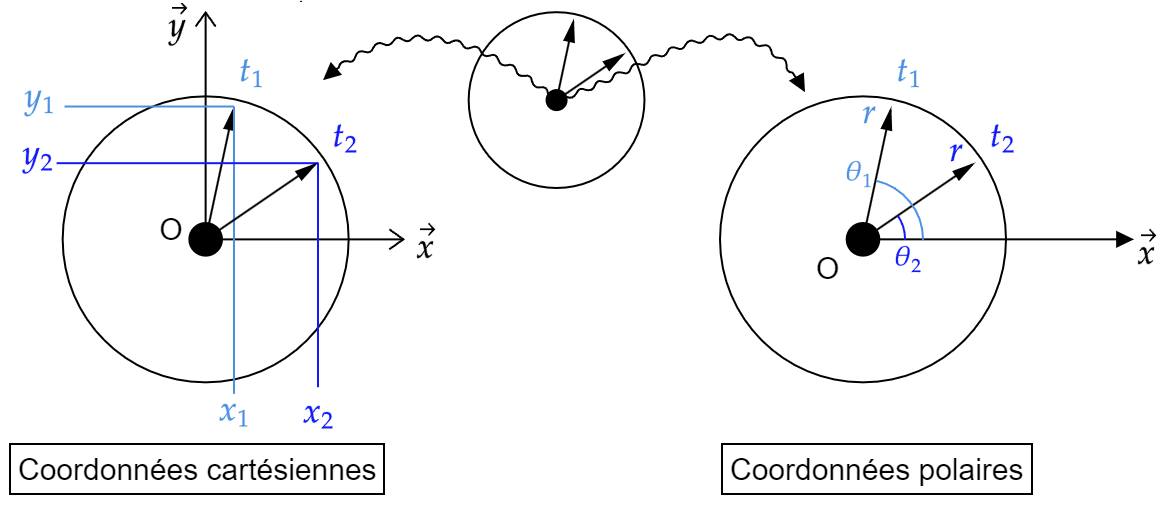
\includegraphics[width=1\textwidth]{Images/pol1.png} % Include the figure image
	\caption{Différence entre coordonnées cartésiennes et polaires.}
	\label{pol1} % Unique label used for referencing the figure in-text
\end{figure}

Sur la figure [\ref{pol1}], en coordonnées cartésiennes, le bout de l'aiguille en $t_1$ a pour coordonnées ($x_1; y_1$) et pour $t_2$ ($x_2 ; y_2$) : les \textbf{deux} valeurs changent. 
En coordonnées polaires, le bout de l'aiguille en $t_1$ a pour coordonnées ($r ; \theta_1$) et pour $t_2$ ($r ; \theta_2 $) : \textbf{Une} seule valeur est changée.

Pour le cas général, les coordonnées polaires se représentent comme sur la figure [\ref{pol2}]

\begin{figure}[H] % Use [H] to suppress floating and place the figure/table exactly where it is specified in the text
	\centering % Horizontally center the figure on the page
	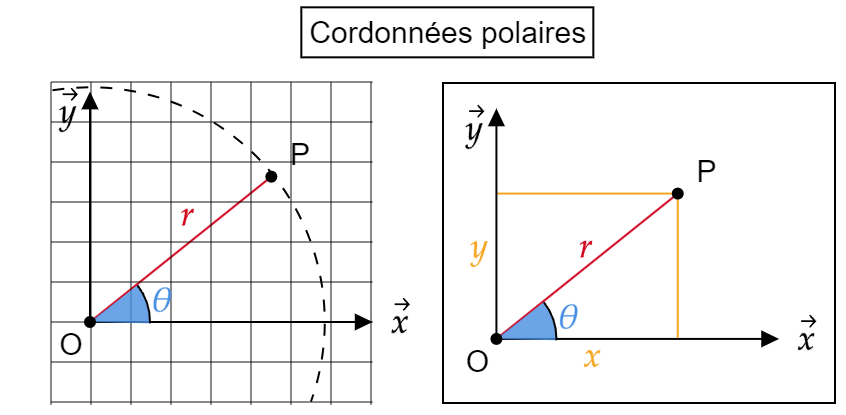
\includegraphics[width=1\textwidth]{Images/pol2.png} % Include the figure image
	\caption{Coordonnées polaires.}
	\label{pol2} % Unique label used for referencing the figure in-text
\end{figure}
\begin{Exercice}
    D'après la figure [\ref{pol2}] essayez d'exprimer $r$ en fonction de $x$ et $y$. Pensez aux formules trigonométriques.

%%%%%%%%%%%%%%%%%%%%%%%%%%%%%%%%%%%%%%%%%%%%%%%%%%%%%%%%%%%%%%%%%%%%%%%%%%%%%%%%%

\tikzset{every picture/.style={line width=0.75pt}} %set default line width to 0.75pt        

\begin{tikzpicture}[x=0.75pt,y=0.75pt,yscale=-1,xscale=1]
%uncomment if require: \path (0,142); %set diagram left start at 0, and has height of 142

%Straight Lines [id:da8668537732864932] 
\draw [color={rgb, 255:red, 245; green, 166; blue, 35 }  ,draw opacity=1 ]   (109.38,48.29) -- (19,48.29) ;
%Straight Lines [id:da04240430164333486] 
\draw [color={rgb, 255:red, 208; green, 2; blue, 27 }  ,draw opacity=1 ]   (109.38,48.29) -- (18.71,120.96) ;
%Straight Lines [id:da4411439485257207] 
\draw    (18.71,120.96) -- (157.04,120.96) ;
\draw [shift={(160.04,120.96)}, rotate = 180] [fill={rgb, 255:red, 0; green, 0; blue, 0 }  ][line width=0.08]  [draw opacity=0] (8.93,-4.29) -- (0,0) -- (8.93,4.29) -- cycle    ;
%Shape: Arc [id:dp8727987582575247] 
\draw  [draw opacity=0][fill={rgb, 255:red, 74; green, 144; blue, 226 }  ,fill opacity=0.81 ] (42.42,102.58) .. controls (46.36,107.66) and (48.71,114.03) .. (48.71,120.96) .. controls (48.71,121.18) and (48.71,121.41) .. (48.7,121.63) -- (18.71,120.96) -- cycle ; \draw   (42.42,102.58) .. controls (46.36,107.66) and (48.71,114.03) .. (48.71,120.96) .. controls (48.71,121.18) and (48.71,121.41) .. (48.7,121.63) ;  
%Shape: Circle [id:dp36815487674584846] 
\draw  [fill={rgb, 255:red, 0; green, 0; blue, 0 }  ,fill opacity=1 ] (16.21,120.96) .. controls (16.21,119.58) and (17.33,118.46) .. (18.71,118.46) .. controls (20.09,118.46) and (21.21,119.58) .. (21.21,120.96) .. controls (21.21,122.34) and (20.09,123.46) .. (18.71,123.46) .. controls (17.33,123.46) and (16.21,122.34) .. (16.21,120.96) -- cycle ;
%Straight Lines [id:da546920544152073] 
\draw    (18.71,120.96) -- (18.71,8.72) ;
\draw [shift={(18.71,5.72)}, rotate = 90] [fill={rgb, 255:red, 0; green, 0; blue, 0 }  ][line width=0.08]  [draw opacity=0] (8.93,-4.29) -- (0,0) -- (8.93,4.29) -- cycle    ;
%Straight Lines [id:da9819027378108172] 
\draw [color={rgb, 255:red, 245; green, 166; blue, 35 }  ,draw opacity=1 ]   (109.38,48.29) -- (109.38,120.43) ;
%Shape: Circle [id:dp33757938500758367] 
\draw  [fill={rgb, 255:red, 0; green, 0; blue, 0 }  ,fill opacity=1 ] (106.88,48.29) .. controls (106.88,46.91) and (107.99,45.79) .. (109.38,45.79) .. controls (110.76,45.79) and (111.88,46.91) .. (111.88,48.29) .. controls (111.88,49.67) and (110.76,50.79) .. (109.38,50.79) .. controls (107.99,50.79) and (106.88,49.67) .. (106.88,48.29) -- cycle ;

% Text Node
\draw (2.38,123.62) node [anchor=north west][inner sep=0.75pt]   [align=left] {O};
% Text Node
\draw (117.71,28.29) node [anchor=north west][inner sep=0.75pt]   [align=left] {P};
% Text Node
\draw (168.38,109.69) node [anchor=north west][inner sep=0.75pt]    {$\vec{x}$};
% Text Node
\draw (59.04,65.13) node [anchor=north west][inner sep=0.75pt]  [color={rgb, 255:red, 208; green, 2; blue, 27 }  ,opacity=1 ] [align=left] {$\displaystyle r$};
% Text Node
\draw (48.38,100.63) node [anchor=north west][inner sep=0.75pt]  [color={rgb, 255:red, 74; green, 144; blue, 226 }  ,opacity=1 ] [align=left] {$\displaystyle \theta $};
% Text Node
\draw (2.38,4.69) node [anchor=north west][inner sep=0.75pt]    {$\vec{y}$};
% Text Node
\draw (61.38,120.19) node [anchor=north west][inner sep=0.75pt]  [color={rgb, 255:red, 245; green, 166; blue, 35 }  ,opacity=1 ]  {$x$};
% Text Node
\draw (4.88,65.69) node [anchor=north west][inner sep=0.75pt]  [color={rgb, 255:red, 245; green, 166; blue, 35 }  ,opacity=1 ]  {$y$};
% Text Node
\draw (202.96,12.13) node [anchor=north west][inner sep=0.75pt]  [color={rgb, 255:red, 208; green, 2; blue, 27 }  ,opacity=1 ] [align=left] {$\displaystyle r=$};
% Text Node
\draw (201.96,60.9) node [anchor=north west][inner sep=0.75pt]  [color={rgb, 255:red, 245; green, 166; blue, 35 }  ,opacity=1 ]  {$x=$};
% Text Node
\draw (201.96,112.69) node [anchor=north west][inner sep=0.75pt]  [color={rgb, 255:red, 245; green, 166; blue, 35 }  ,opacity=1 ]  {$y=$};
% Text Node
\draw (400.21,4.79) node [anchor=north west][inner sep=0.75pt]   [align=left] {$\displaystyle \overrightarrow{OP} =$};


\end{tikzpicture}
%%%%%%%%%%%%%%%%%%%%%%%%%%%%%%%%%%%%%%%%%%%%%%%%%%%%%%%%%%%%%%%%%%%%%%%%%

    
\end{Exercice}

\subsection{Coordonnées cylindriques}

Les coordonnées cylindriques sont une extension des coordonnées polaires. On fait une succession d'une infinité de plans des coordonnées polaires pour remplir un cylindre. Comme pour les coordonnées polaires, les coordonnées cylindriques sont souvent utilisées lorsque le problème traité présente une symétrie de révolution autour d’un axe, avec lequel sera confondu l’un des vecteurs de la base. Pour étudier les mouvements sur un tour, c'est le système de coordonnées idéal.

\begin{figure}[H] % Use [H] to suppress floating and place the figure/table exactly where it is specified in the text
	\centering % Horizontally center the figure on the page
	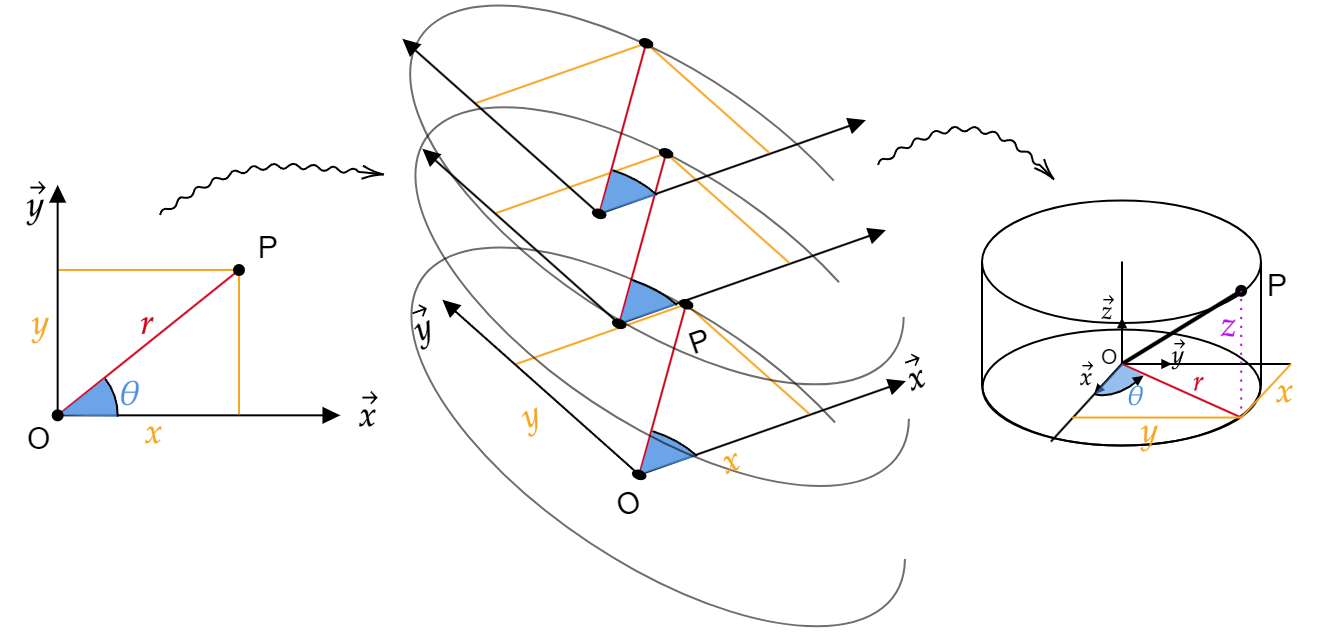
\includegraphics[width=1\textwidth]{Images/cyl1.png} % Include the figure image
	\caption{Changement des coordonnées polaires en cylindriques.}
	\label{cyl1} % Unique label used for referencing the figure in-text
\end{figure}

On cherche à connaître la distance $\Vec{OP}$ en coordonnées cylindriques. Par rapport au coordonnées polaires, il y a toujours $r$, et maintenant il faut ajouter la "hauteur" sur l'axe $\Vec{z}$. Ici, $r$ nous donne le rayon, et $z$ la "longueur".


\begin{figure}[H] % Use [H] to suppress floating and place the figure/table exactly where it is specified in the text
	\centering % Horizontally center the figure on the page
	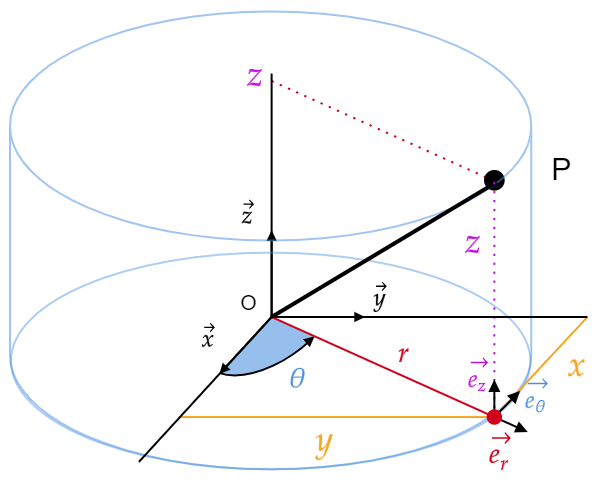
\includegraphics[width=0.9\textwidth]{Images/cyl3.png} % Include the figure image
	\caption{Représentation des coordonnées cylindriques.}
	\label{cyl3} % Unique label used for referencing the figure in-text
\end{figure}

La distance $\Vec{OP}$ dépendra du diamètre $r$ et de la hauteur $z$ :\\
\begin{center}
$\Vec{OP}=r\Vec{e_r}+z\Vec{e_z}$
\end{center}
Le vecteur unitaire $\Vec{e_r}$ change de direction en fonction de l'angle $\theta$, plus besoin des coordonnées $x$ et $y$. \\
\noindent On peut passer du système cylindrique au système cartésien :
$\begin{cases}
x=r.\cos( \theta )\\
y=r.\sin( \theta )\\
z=z
\end{cases}$





\section{Conclusion}

Pour étudier le mouvement des outils et des pièces dans l'espace, nous avons le choix du système de coordonnée. En fonction du besoin (forme, trajectoire, symétries) dépendra le système de coordonnée choisi. La plupart du temps, vous travaillerez avec le système de coordonnées cartésien. 

\begin{figure}[H] % Use [H] to suppress floating and place the figure/table exactly where it is specified in the text
	\centering % Horizontally center the figure on the page
	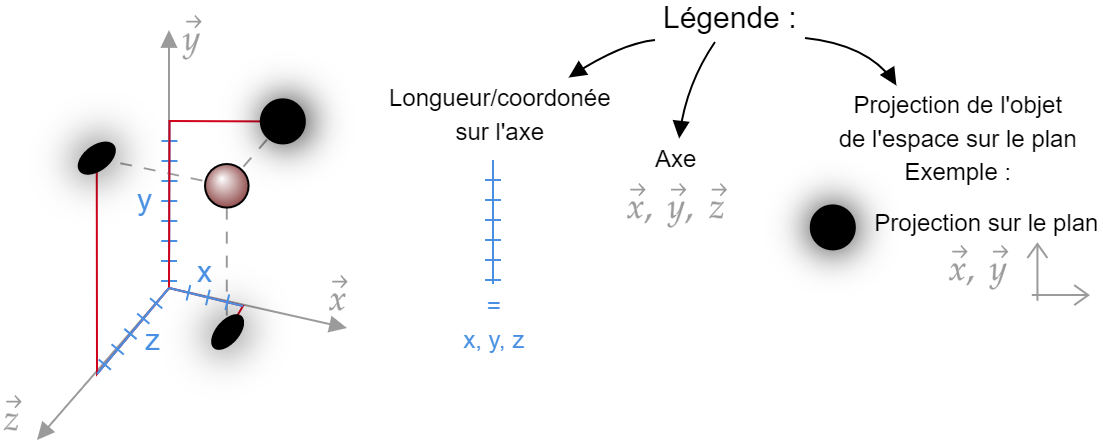
\includegraphics[width=0.9\textwidth]{Images/coord10.png} % Include the figure image
	\caption{Représentation des coordonnées cartésienne : résumé.}
	\label{coord10} % Unique label used for referencing the figure in-text
\end{figure}


%----------------------------------------------------------------------------------------
%	PRESENTING INFORMATION/RESULTS EXAMPLES CHAPTER
%----------------------------------------------------------------------------------------

\chapterimage{Images/chapt_F.jpg} % Chapter heading image
\chapterspaceabove{6.25cm} % Whitespace from the top of the page to the chapter title on chapter pages
\chapterspacebelow{7.5cm} % Amount of vertical whitespace from the top margin to the start of the text on chapter pages

%------------------------------------------------
\chapter{Représenter le réel}

\section{Introduction}
Nous savons maintenant exprimer la position de points dans l'espace. Cela nous permets de programmer une succession de point pour avoir une trajectoire d'outil par exemple. Aussi, pour le bon usinage d'une pièce, il est essentiel de connaître d'autres indicateurs comme la vitesse d'outil ou de la pièce, les accélérations et les actions mécaniques (efforts, forces, etc.) générées dans la machine.

\begin{figure}[H]  % Use [H] to suppress floating and place the figure/table exactly where it is specified in the text
	\centering % Horizontally center the figure on the page
 \fbox{
	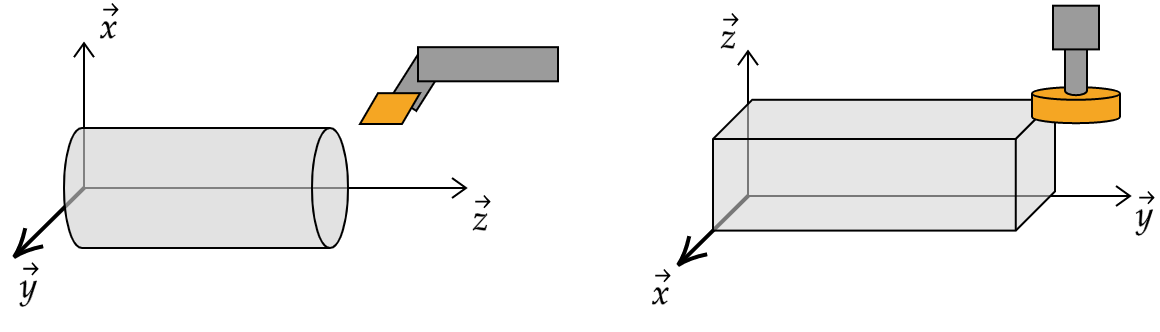
\includegraphics[width=0.9\textwidth]{Images/reel1.png} } % Include the figure image
\end{figure}

Vous vous en doutez, il est indispensable de connaître les efforts engendrés par l'outil pour s'assurer un enlèvement de copeaux ni trop brutal ni trop faible. On doit toujours garder à l'esprit que la machine ne fera que ce qu'on lui demande. On peu facilement casser l'outil ou la pièce et même rendre la machine totalement hors service.

Nous allons apprendre à représenter les différents éléments incontournables pour les sciences de l'ingénieur et notamment pour la conception préliminaire.







\subsection{Notation vectorielle}
Les systèmes de coordonnées sont construit grâce à notre bibliothèque de vecteurs. Pour représenter d'autres éléments, nous utiliserons encore des vecteurs. Ils nous permettent d'exprimer une direction et un sens par rapport à notre repère. Pour utiliser un vecteur, on met simplement une flèche au dessus de ce qu'on écrit, cela veut dire qu'il à plusieurs \textit{composantes}\footnote{Un vecteur inséré dans un repère à trois dimensions (trois axes) pourra être décomposé en trois valeurs : trois composantes.}.\\

\begin{definition}\label{Vecteurs}
    Un vecteur $\Vec{u}$ est défini par :
    \begin{itemize}
        \item Une direction ;
        \item Un sens ;
        \item Une longueur (sa norme).
    \end{itemize}
Un vecteur est indépendant du point d’origine.

\begin{figure}[H] % Use [H] to suppress floating and place the figure/table exactly where it is specified in the text
	\centering % Horizontally center the figure on the page
	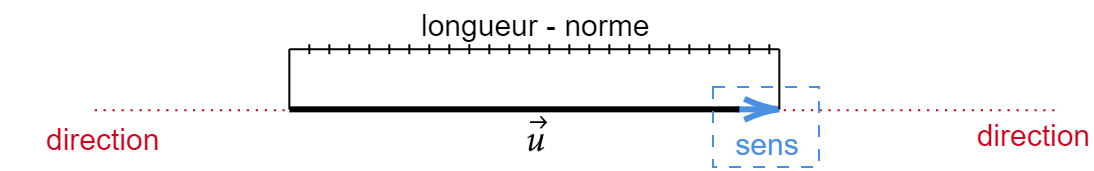
\includegraphics[width=0.9\textwidth]{Images/reel2.png} % Include the figure image
	\caption{Représentation d'un vecteur.}
	\label{vecteur} % Unique label used for referencing the figure in-text
\end{figure}

\end{definition}

Exemple d'écriture de vecteur : \\
$\overrightarrow{Vecteur}$ ;  $\overrightarrow{Vent}=\ \begin{Bmatrix} 10\\ 5 \\ -13 \end{Bmatrix} $ ; $\overrightarrow{W}$



Pour noter la longueur d'un vecteur (sa norme) on écrit : $\Vert \overrightarrow{Vecteur}\Vert \ $

Pour n'importe quel vecteur, on calcul sa norme grâce à ses composantes. Si $ \overrightarrow{u} = a \vec{x} + b \vec{y} + c \vec{z} \ $, la norme d'un vecteur est égale à :\\
$\Vert \overrightarrow{u}\Vert =\ \sqrt{a^2 + b^2 + c^2} $

\begin{figure}[H] % Use [H] to suppress floating and place the figure/table exactly where it is specified in the text
	\centering % Horizontally center the figure on the page
	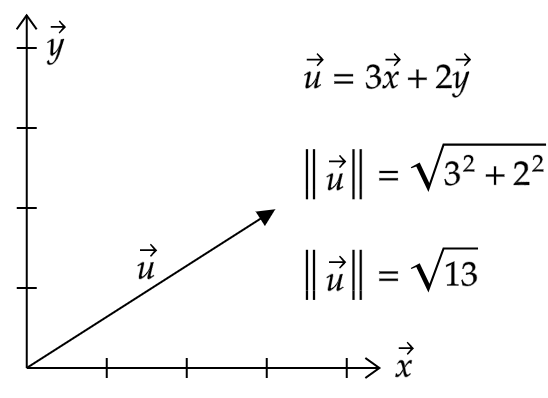
\includegraphics[width=0.6\textwidth]{Images/norme3.png} % Include the figure image
	\caption{Calcul de la norme d'un vecteur.}
	\label{norme3} % Unique label used for referencing the figure in-text
\end{figure}


\begin{Exercice}
    Calculez la norme des vecteurs suivants :\\
    \begin{itemize}
        \item $\vec{u} =8\vec{x} +4\vec{y} + \vec{z}$
        \item $\overrightarrow{w} =-\vec{x} +6\vec{y} - 2\vec{z}$
        \item $\overrightarrow{OP} = \vec{v} + \vec{w} $ 
    
    \end{itemize}


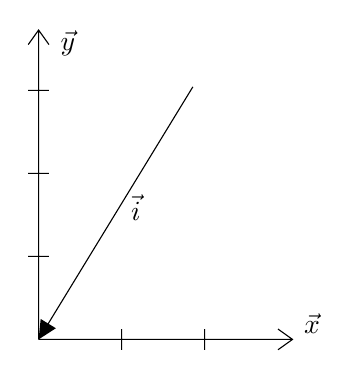
\begin{tikzpicture}[x=0.75pt,y=0.75pt,yscale=-1,xscale=1]
%uncomment if require: \path (0,166); %set diagram left start at 0, and has height of 166

%Shape: Axis 2D [id:dp9182153345792954] 
\draw  (12,154) -- (134.33,154)(12,4.95) -- (12,154) -- cycle (127.33,149) -- (134.33,154) -- (127.33,159) (7,11.95) -- (12,4.95) -- (17,11.95) (52,149) -- (52,159)(92,149) -- (92,159)(7,114) -- (17,114)(7,74) -- (17,74)(7,34) -- (17,34) ;
\draw   ;
%Straight Lines [id:da0676112765377892] 
\draw    (86.33,32.29) -- (13.56,151.44) ;
\draw [shift={(12,154)}, rotate = 301.41] [fill={rgb, 255:red, 0; green, 0; blue, 0 }  ][line width=0.08]  [draw opacity=0] (8.93,-4.29) -- (0,0) -- (8.93,4.29) -- cycle    ;

% Text Node
\draw (55.33,83.07) node [anchor=north west][inner sep=0.75pt]    {$\vec{i}$};
% Text Node
\draw (138.67,140.4) node [anchor=north west][inner sep=0.75pt]    {$\vec{x}$};
% Text Node
\draw (21.33,4.07) node [anchor=north west][inner sep=0.75pt]    {$\vec{y}$};


\end{tikzpicture}



\end{Exercice}

\begin{remark}
    Attention, il ne faut pas confondre la position des points et un vecteur qui peut y être associé. On peut construire un vecteur avec la position d'un point et d'une origine, ou de deux points.

    \begin{figure}[H] % Use [H] to suppress floating and place the figure/table exactly where it is specified in the text
	\centering % Horizontally center the figure on the page
	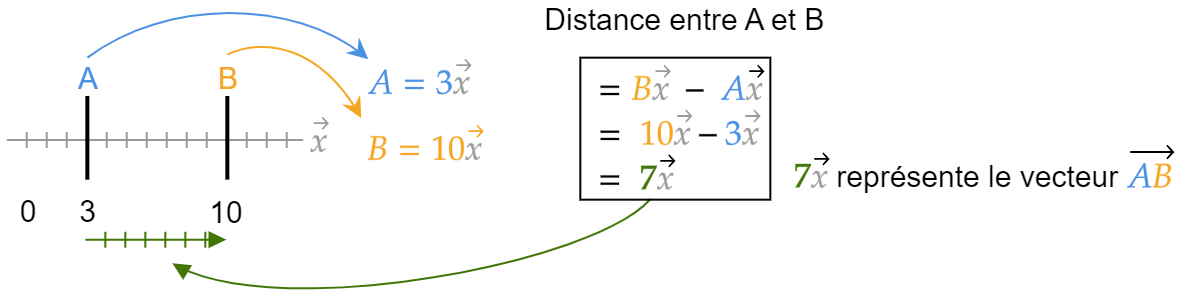
\includegraphics[width=1\textwidth]{Images/pos1.png} % Include the figure image
\end{figure}
   
\end{remark}




\section{Vitesse et accélération}
Nous savons nous servir des vecteurs pour représenter la position d'un point par rapport à un repère. Maintenant, nous allons voir 


\subsection{Vecteur trajectoire}

\section{Forces}
On écrivait comme ça,  $\Vec{i}=\ \begin{Bmatrix} a\\ b \\ c \end{Bmatrix} $  maintenant faut écrire comme ça 
 {$\overrightarrow{\mathcal{F}_{moteur}} =\ \begin{Bmatrix}
F_{x}\\
F_{y}\\
F_{z}
\end{Bmatrix}_{( \mathcal{B}_{1} ,\ \vec{x} ,\ \vec{y} ,\vec{z})}$};

2D , 3D, certain sont constant $\overrightarrow{\mathcal{V}_{(train\rightarrow route)}} \ =\ C^{te}$ d'autre non. $\overrightarrow{\mathcal{T}_{(train\rightarrow route)}} \ =\ X$ trajectoire

\section{Moments / Couples}
 (double fleche pour les moments) 






\subsection{Notation de Torseurs}


Pour aller plus loin sur les tenseurs : \url{https://www.youtube.com/watch?v=zPRbbM4KJBY&t=1066s}

\begin{Extrait}\index{Torseurs (exercice)}
TS CPRP 2015 \\
On se propose d’estimer l’effort maxi que doit appliquer la contre-pointe sur le papillon lors de l’opération de perçage. \\



\noindent \begin{minipage}{0.5\textwidth}
\vspace{1cm}
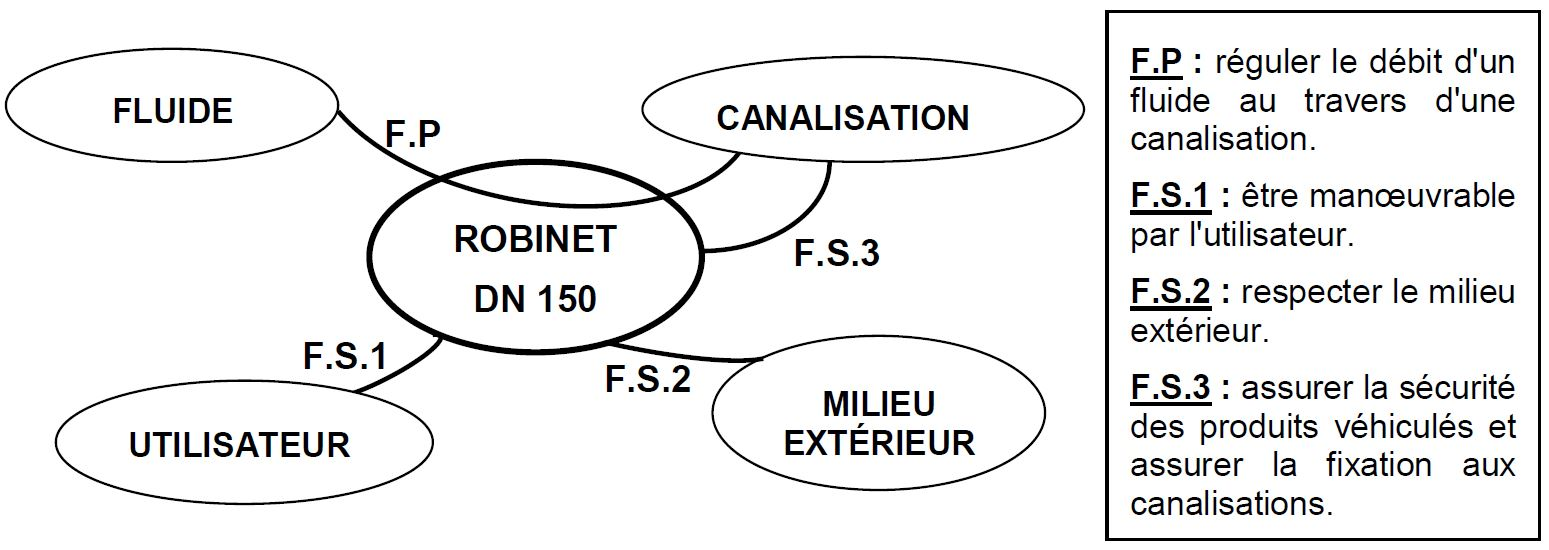
\includegraphics[width=1\textwidth]{Images/2015.JPG}
\label{fig:nature}
\end{minipage}
\hspace{0.05\textwidth}
\begin{minipage}{0.4\textwidth}
Hypothèses : 
\begin{itemize}
\item Le problème possède un plan de
symétrie mécanique ($\mathcal{B}, \Vec{y}, \Vec{z}$) ;
\item L’ensemble des contacts entre
solide se fait avec adhérence. On
prendra $tan(\phi_{0}) = 0,1.$ ;
\item L’étude est menée à la « limite du
glissement »;
\item L'action de la pesanteur est
négligée ;
\item Pour l’étude, l’effort de pénétration notée $\overrightarrow{\mathcal{A}_{(f\rightarrow p)}}\ $ aura une intensité de : \\ $ \Vert \overrightarrow{\mathcal{A}_{(f\rightarrow p)}} \Vert = 2000 N\ $
\end{itemize}

\end{minipage}


On notera :
$\displaystyle \begin{Bmatrix}
A_{f\rightarrow p}
\end{Bmatrix} =\begin{Bmatrix}
\overrightarrow{A_{f\rightarrow p}} =2000.\vec{y} & \\
\overrightarrow{\mathcal{M}_{A}{}_{\left( f\rightarrow p\right)}} =\vec{0} & 
\end{Bmatrix}_{A,\ (\mathcal{R} ,\ \vec{x} ,\ \vec{y} ,\ \vec{z})}$

Concernant l’action de posage, on considère que la liaison entre les supports à bille
oscillante et le papillon est une liaison appui plan. En l’absence de mouvement, le
torseur modélisant l’action mécanique transmissible comporte 3 inconnues Yc, Zc et Lc.
Comme la liaison est unilatérale, ZC > 0.

$\displaystyle \begin{Bmatrix}
C_{pp\rightarrow papillon}
\end{Bmatrix} =\begin{Bmatrix}
0 & L_{c}\\
Y_{c} & 0\\
Z_{c} & 0
\end{Bmatrix}_{C,\ (\mathcal{R} ,\ \vec{x} ,\ \vec{y} ,\ \vec{z})} avec\ Y_{c} =Z_{c} .\tan( \phi_{0})$


\end{Extrait}




 
\section{Notations}

\begin{definition}\index{Solide indéformable}
Un solide $\mathcal{S}$ est appelé indéformable s'il est caractérisé par un ensemble de points et que la distance entre deux points reste invariante au cours du temps. Mathématiquement, on écrit :


    $ \forall \ t,\forall A\ \in S,\ \forall B\ \in S\ :\ \Vert \overrightarrow{AB}\Vert =C^{cte} \ $ 


\textit{On lit la ligne du dessus comme suit :} Quelque chose est un solide si, pour tout instant $t$, pour tous points $A$ d'un solide $\mathcal{S}$, pour tout point $B$ appartenant aussi à $\mathcal{S}$, la distance entre les points $A$ et $B$ reste constant au cours du temps.
\end{definition}



\begin{corollary}[S2.4] 
aze
\end{corollary}

\begin{definition}{Normes}\index{Norme}
aze
\end{definition}

\begin{theorem}
    sqdf
\end{theorem}

\begin{remark}
    aze
\end{remark}






%----------------------------------------------------------------------------------------
%	PRESENTING INFORMATION/RESULTS EXAMPLES CHAPTER
%----------------------------------------------------------------------------------------

\chapterimage{Images/A6.jpg} % Chapter heading image
\chapterspaceabove{6.25cm} % Whitespace from the top of the page to the chapter title on chapter pages
\chapterspacebelow{7.5cm} % Amount of vertical whitespace from the top margin to the start of the text on chapter pages

%------------------------------------------------


	




\newpage
\section{ANNEXE}


\phantomsection
\addcontentsline{toc}{chapter}{\textcolor{ocre}{Index}} % Add an Index heading to the table of contents
\printindex % Output the index


\end{document}


